\documentclass{article}

% NeurIPS 2026 main-track double-blind submission.
\usepackage{neurips_2026}

% Encoding & fonts
\usepackage[utf8]{inputenc}
\usepackage[T1]{fontenc}
\usepackage{microtype}
\usepackage{comment}

% Math
\usepackage{amsmath}
\usepackage{amssymb}
\usepackage{amsthm}
\usepackage{amsfonts}
\usepackage{mathtools}
\usepackage{nicefrac}
\usepackage{bm}

% Floats
\usepackage{graphicx}
\usepackage{booktabs}
\usepackage{threeparttable}
\usepackage{subcaption}
\usepackage{xcolor}

% Algorithms
\usepackage{algorithm}
\usepackage{algpseudocode}

% Lists
\usepackage{enumitem}

% Hyperref + cleveref (cleveref must be loaded last among ref packages)
\usepackage{hyperref}
\usepackage{url}
\usepackage[capitalize,noabbrev]{cleveref}

% --- Theorem environments (shared counter, scoped to section) ---
\theoremstyle{plain}
\newtheorem{theorem}{Theorem}[section]
\newtheorem{proposition}[theorem]{Proposition}
\newtheorem{lemma}[theorem]{Lemma}
\newtheorem{corollary}[theorem]{Corollary}

\theoremstyle{definition}
\newtheorem{definition}[theorem]{Definition}
\newtheorem{assumption}[theorem]{Assumption}

\theoremstyle{remark}
\newtheorem{remark}[theorem]{Remark}

% Cleveref names
\crefname{theorem}{Theorem}{Theorems}
\crefname{proposition}{Proposition}{Propositions}
\crefname{lemma}{Lemma}{Lemmas}
\crefname{corollary}{Corollary}{Corollaries}
\crefname{assumption}{Assumption}{Assumptions}
\crefname{algorithm}{Algorithm}{Algorithms}
\crefname{equation}{Eq.}{Eqs.}
\crefname{section}{Section}{Sections}
\crefname{subsection}{Section}{Sections}
\crefname{appendix}{Appendix}{Appendices}
\crefname{figure}{Figure}{Figures}
\crefname{table}{Table}{Tables}

% Convenience macros
\DeclareMathOperator{\Var}{Var}
\DeclareMathOperator{\Cov}{Cov}
\DeclareMathOperator{\MSE}{MSE}
\DeclareMathOperator*{\argmin}{arg\,min}
\DeclareMathOperator*{\argmax}{arg\,max}
\newcommand{\E}{\mathbb{E}}
\newcommand{\Prob}{\mathbb{P}}
\newcommand{\R}{\mathbb{R}}
\newcommand{\1}{\mathbf{1}}

% --- Title ---
\title{Optimal Real-Data Allocation for\\Synthetic-Data-Augmented Inference}

% Anonymous author block for double-blind submission.
\author{%
  Sikun Xu \\ Olin Business School \\ Washington University in St.~Louis \\ St.~Louis, MO 63130 \\ \texttt{sikun@wustl.edu} \\
  \And
  Zineng Xu \\ National University of Singapore \\ \texttt{XXX@XXX.edu} \\
  \And
Mingduo Zhao \\ University of California, Berkeley \\ \texttt{XXX@XXX.edu}\\ }

\begin{document}

\maketitle

\begin{abstract}
  Large language models have made synthetic data inexpensive, but they can still be biased. When real data are scarce, researchers must decide how much of the real sample to use for direct estimation and how much to spend calibrating the generator. We study this allocation problem and derive the marginal-value condition for the optimal calibration size: $(v_n + c x^{-2\beta})^2 = 2\beta a c x^{-(2\beta+1)}$, where $x$ is the calibration size, $v_n$ is synthetic sampling variance, $a$ is the real-estimator variance constant, and $c x^{-2\beta}$ is squared synthetic bias. This condition has no universal fixed-share solution and yields five allocation regimes. In the main regime, $m_n \asymp n$ and $\beta > 1/2$, the optimal calibration size grows only as $n^{2/(2\beta+1)}$, so the calibration share vanishes; rules that keep a positive fixed fraction of real observations in calibration over-calibrate asymptotically. We also propose an adaptive grid estimator with an oracle inequality and a safety check, $xB_n(x)<a$, that falls back to all-real estimation when synthetic data cannot help. Across approximately $10^7$ Monte Carlo replications, the corrected oracle reduces MSE by about $47\%$ relative to all-real estimation in the headline cell, compared with about $22\%$ for a fixed-share baseline. For inference, naive Wald intervals around the MSE-optimal estimator can undercover, while validation debiasing substantially restores coverage. These results provide guidance for when synthetic data are useful, how much real data should be used to make them reliable, and how to conduct valid inference with synthetic-data-augmented estimators.

\end{abstract}

\section{Introduction}
% POLISHED
\label{sec:intro}

Large language models have made synthetic data cheap. A single generator can now produce millions of labeled examples, simulated outcomes, or auxiliary observations on demand \citep{kaplan2020scaling,hoffmann2022chinchilla}. This is valuable when real data are expensive, sensitive, slow to collect, or constrained by institutions. But abundance does not remove the empirical bottleneck: synthetic observations come from a model, and that model may preserve bias, misspecified structure, or distortions inherited from training and alignment. The central question is therefore not whether synthetic data can be generated, but how much scarce real data should be spent making them reliable.

We study this question as a real-data allocation problem. A researcher wants to estimate a scalar parameter $\theta^\star$ of a real population, such as a treatment effect, a mean, or a regression coefficient, and has a budget of $n$ real observations. Each observation can be used as direct evidence about $\theta^\star$ or as calibration data that makes future synthetic draws less biased. Calibration improves the artificial data-generating process, but it also reduces the real sample left for direct estimation. This is a Neyman-style allocation problem \citep{neyman1934}, except the split is across uses of data rather than across strata.

A tempting shortcut is to choose the calibration share as a fixed function of the bias-decay exponent. That shortcut misses a second force in the problem. Under a power-law squared-bias curve $b_2(x) \asymp c x^{-2\beta}$, where $x$ is the calibration size and $\beta$ is the bias-decay exponent, the synthetic estimator also has sampling variance $v_n=\sigma_S^2/m_n$. The relevant synthetic error is therefore $B_n(x)=v_n+cx^{-2\beta}$, not the bias term alone.

Keeping this term changes the allocation logic. The researcher must ask whether one more calibration observation reduces synthetic error enough to justify the lost real-estimation precision. This marginal-value comparison yields the first-order condition
\[
  (v_n+c x^{-2\beta})^2 = 2\beta a c x^{-(2\beta+1)}.
\]
When the synthetic budget grows with the real budget, $m_n \asymp n^\rho$, and generator bias declines faster than the parametric rate, $\beta>1/2$, this condition often calls for sublinear calibration. In the leading case $m_n\asymp n$, the optimal calibration share goes to zero even though the number of calibration observations diverges. Positive fixed-share rules therefore over-calibrate in this regime.

Existing literatures stop one step before the allocation problem created by synthetic data. Neyman allocation optimizes sampling across strata \citep{neyman1934,cochran1977}; here the split is across \emph{uses} of the same scarce real observations. Shrinkage and model-combination methods choose weights after estimators exist \citep{stein1956,jamesstein1961,hansen2007combination}; they do not decide how much real data should be spent making a biased synthetic estimator usable. Double machine learning and prediction-powered inference correct bias under fixed splitting rules \citep{chernozhukov2018doubleml,angelopoulos2023ppi,zrnic2024crosspp}; they do not supply the marginal-value condition for calibration itself. Transfer and auxiliary-data learning treat the outside source as given \citep{panyang2010transfer,bastani2021proxy,licaili2022transfer}, while neural scaling laws describe how models improve with data \citep{kaplan2020scaling,hoffmann2022chinchilla}. Our contribution is to turn these pieces into a real-data allocation theory: a corrected first-order condition, its phase diagram, and inference rules built on standard semiparametric machinery \citep{bickelklaassenritovwellner1993,vandervaart1998asymptotic}.

Our contributions are as follows:
\begin{itemize}[leftmargin=*]
  \item \textbf{Corrected allocation condition.} For any interior optimum $x^\star$ of the profiled mean-squared error, the calibration size satisfies
    $(v_n + c x^{-2\beta})^2 = 2\beta a c x^{-(2\beta+1)}$,
    where $a$ is the real-estimator variance constant and $c x^{-2\beta}$ is squared synthetic bias. This condition keeps the synthetic-variance term omitted by fixed-share shortcuts.

  \item \textbf{Phase diagram.} We characterize five allocation regimes indexed by the bias-decay exponent $\beta$ and the synthetic-budget exponent $\rho$. In the headline regime, $\beta>1/2$ and $0<\rho<\beta+1/2$, the optimal calibration size is $x_n^\star \asymp n^{2\rho/(2\beta+1)}$, so the share $\lambda_n^\star=x_n^\star/n$ vanishes. When $\rho=1$, this reduces to $x_n^\star \asymp n^{2/(2\beta+1)}$: even linear synthetic scale calls for sublinear real-data calibration.

  \item \textbf{Adaptive implementation.} We give a grid estimator that learns the bias-decay curve on a held-out pilot grid, minimizes the corrected profiled risk over interior and boundary choices $x=0,n$, and applies the safety check $x \cdot B_n(x) < a$ before using synthetic data. Under uniform consistency of the pilot risk estimates, the adaptive estimator matches the oracle in relative risk.

  \item \textbf{Inference and evidence.} We separate MSE-optimal point estimation from valid inference. The mixed estimator can reduce point risk while leaving enough residual synthetic bias to make naive Wald intervals undercover; validation debiasing restores coverage at a variance cost, in the spirit of double machine learning and prediction-powered inference \citep{chernozhukov2018doubleml,angelopoulos2023ppi}. Across roughly $10^7$ Monte Carlo replications, the corrected oracle attains MSE $0.535$ relative to all-real estimation in the headline cell, compared with $0.779$ for a fixed-share baseline. In Experiment~4, validation-debiased intervals raise worst-cell coverage from $0.855$ to $0.938$ at the nominal $0.95$ level.
\end{itemize}

The rest of the paper proceeds as follows. Section~\ref{sec:setup} introduces the setup and notation. Section~\ref{sec:mixing} derives the optimal-mixing identity and corrected first-order condition. Section~\ref{sec:phase} gives the phase diagram. Section~\ref{sec:adaptive} develops the adaptive algorithm and inference results. Section~\ref{sec:experiments} reports the simulations, and Section~\ref{sec:discussion} concludes.


\section{Setup}
\label{sec:setup}

\paragraph{Estimand and observables.}
Fix a probability space and a measurable sample space $\mathcal{X}$. Let $P^*$ be the real data-generating distribution. Let $\theta:\mathcal{P}\to\mathbb{R}$ be a scalar functional defined on a class $\mathcal{P}$ of distributions on $\mathcal{X}$ that contains $P^*$ and the synthetic distributions introduced below. The target is $\theta^*:=\theta(P^*)$. The researcher observes a real sample
\begin{equation*}
X_1,\dots,X_n \stackrel{\mathrm{iid}}{\sim} P^*,
\end{equation*}
where $n$ is the total real-data budget. The researcher chooses an integer calibration budget $x\in\{0,1,\dots,n\}$ and splits $[n]:=\{1,\dots,n\}$ into a \emph{calibration set} $C_x\subset[n]$ with $|C_x|=x$ and an \emph{estimation set} $E_x:=[n]\setminus C_x$ with $|E_x|=n_e:=n-x$. The calibration share is $\lambda := x/n\in[0,1]$. We enforce sample splitting throughout: estimators use only their assigned subsets, and the partition is independent of $\{X_i\}$. Let $\mathcal{F}_C := \sigma(\{X_i\}_{i\in C_x})$ denote the information in the calibration set. Intuitively, $C_x$ is the data the generator learns from, and $E_x$ is the data held back for direct estimation of $\theta^*$.

\paragraph{Generator and synthetic estimator.}
A \emph{calibration map} $\mathcal{G}$ takes the calibration sample $\{X_i\}_{i\in C_x}$ and produces a calibrated synthetic distribution $P_x$. Conditionally on $\mathcal{F}_C$, draw synthetic observations
\begin{equation*}
Z_1,\dots,Z_{m_n}\,\bigl|\,\mathcal{F}_C \stackrel{\mathrm{iid}}{\sim} P_x,
\end{equation*}
where $m_n\in\mathbb{N}$ is the synthetic budget. The \emph{pseudo-true} parameter is $\theta_x:=\theta(P_x)$, which is $\mathcal{F}_C$-measurable. The \emph{synthetic bias} is $b(x):=\theta_x-\theta^*$, with second moment $b_2(x):=\mathbb{E}[(\theta_x-\theta^*)^2]$. In words, $b(x)$ measures how far the calibrated generator remains from the real target; spending more real data on calibration should make $b_2(x)$ smaller.

\paragraph{Asymptotic linearity.}
We require the real and synthetic estimators to be $\sqrt{|E_x|}$- and $\sqrt{m_n}$-asymptotically linear, respectively.

\begin{assumption}[Asymptotic linearity of the real estimator]\label{asm:al-real}
There exists a measurable function $\psi:\mathcal{X}\to\mathbb{R}$ with $\mathbb{E}_{P^*}[\psi(X_1)]=0$ and $\mathrm{Var}_{P^*}(\psi(X_1))=a\in(0,\infty)$ such that, for every deterministic sequence of estimation subsets $E\subset[n]$ with $|E|\to\infty$,
\begin{equation*}
\hat\theta_R(E)-\theta^* \;=\; \frac{1}{|E|}\sum_{i\in E}\psi(X_i) \;+\; r_R(E),
\end{equation*}
where the remainder satisfies $\mathbb{E}[r_R(E)]=0$ and $\mathbb{E}[r_R(E)^2]=o(|E|^{-1})$.
\end{assumption}

\begin{assumption}[Asymptotic linearity of the synthetic estimator]\label{asm:al-synth}
There exists a measurable family $(\phi_x)_{x\ge 1}$ such that, conditionally on $\mathcal{F}_C$,
\begin{equation*}
\hat\theta_S(x)-\theta_x \;=\; \frac{1}{m_n}\sum_{j=1}^{m_n}\phi_x(Z_j) \;+\; r_S(x),
\end{equation*}
with $\mathbb{E}[\phi_x(Z_1)\mid\mathcal{F}_C]=0$, $\mathrm{Var}(\phi_x(Z_1)\mid\mathcal{F}_C)=\sigma_S^2(x)$, $\mathbb{E}[r_S(x)\mid\mathcal{F}_C]=0$, and $\mathbb{E}[r_S(x)^2]=o(m_n^{-1})$. Furthermore there is a constant $\sigma_S^2<\infty$ such that $\mathbb{E}[\sigma_S^2(x)]\to\sigma_S^2$ uniformly across the regimes considered.
\end{assumption}

The function $\psi$ is the influence function of $\hat\theta_R$ and $a$ is its variance. Assumption \ref{asm:al-real} delivers the leading-order real-estimator variance
\begin{equation*}
V_R(x)\;:=\;\mathrm{Var}\bigl(\hat\theta_R(E_x)\bigr)\;=\;\frac{a}{n-x}\bigl\{1+o(1)\bigr\},
\end{equation*}
while Assumption \ref{asm:al-synth} gives $\mathrm{Var}(\hat\theta_S(x)\mid\mathcal{F}_C) = \sigma_S^2/m_n + o(m_n^{-1})$. We will write $V_R(x)=a/(n-x)$ and $\mathrm{Var}(\hat\theta_S(x)\mid\mathcal{F}_C) = \sigma_S^2/m_n$ throughout, absorbing the $o(\cdot)$ remainders into the $1+o(1)$ factors that multiply the leading-order risk.

\paragraph{Working model.}
The synthetic-error rate and the synthetic-variance rate are governed by two scalar exponents.

\begin{assumption}[Power-law calibration]\label{asm:pl}
There exist constants $c>0$ and $\beta>0$ such that
\begin{equation*}
b_2(x)\;=\;c\,x^{-2\beta}\bigl\{1+o(1)\bigr\}\qquad\text{as }x\to\infty.
\end{equation*}
\end{assumption}

\begin{assumption}[Synthetic-variance regime]\label{asm:vn}
There exist constants $v_0>0$ and $\rho\ge 0$ such that the synthetic sampling variance $v_n:=\sigma_S^2/m_n$ satisfies
\begin{equation*}
v_n\;=\;v_0\,n^{-\rho}\bigl\{1+o(1)\bigr\}\qquad\text{as }n\to\infty.
\end{equation*}
\end{assumption}

Assumption~\ref{asm:pl} encodes the empirical power-law bias decay often seen in neural scaling-law studies; $\beta$ is the bias-decay exponent and $c$ is the scale. Assumption~\ref{asm:vn} encodes how quickly the synthetic budget grows with the real budget; the main scenario $m_n\asymp n$ corresponds to $\rho=1$. Combining the bias and variance pieces gives the \emph{effective synthetic error}
\begin{equation*}
B_n(x)\;:=\;v_n+c\,x^{-2\beta},
\end{equation*}
which is, up to a $1+o(1)$ factor, the unconditional MSE of $\hat\theta_S(x)$ around $\theta^*$. The first term, $v_n$, is Monte Carlo noise from drawing only $m_n$ synthetic observations. The second term, $c\,x^{-2\beta}$, is residual generator bias after calibration. The allocation problem is to reduce $B_n(x)$ by increasing $x$, while remembering that doing so leaves only $n-x$ real observations for direct estimation.

\paragraph{Linear allocation estimator class.}
For a mixing weight $\alpha\in[0,1]$ and calibration budget $x\in[0,n)$, the \emph{linear allocation estimator} is
\begin{equation}\label{eq:linest}
\hat\theta^{\mathrm{L}}(\alpha,x)\;:=\;\alpha\,\hat\theta_R(E_x)\;+\;(1-\alpha)\,\hat\theta_S(x).
\end{equation}
In words, $\hat\theta^{\mathrm{L}}$ is a convex combination of the real-only estimator on the held-out data and the synthetic-only estimator from the calibrated generator; the two corner cases $\alpha=1$ and $\alpha=0$ recover the all-real estimator on $E_x$ and the synthetic-only estimator, respectively. Section~\ref{sec:mixing} characterizes the optimal $(\alpha,x)$ pair under Assumptions~\ref{asm:al-real},~\ref{asm:al-synth}, ~\ref{asm:pl}, and~\ref{asm:vn}.


% =====================================================================
% POLISHED


\section{Optimal mixing and corrected allocation}
\label{sec:mixing}

This section solves the allocation problem in two steps. First, \Cref{ssec:mixing} fixes the calibration budget $x$ and chooses the best mixing weight $\alpha$ between the real and synthetic estimators. This gives a one-dimensional risk curve $R_n(x)$. Second, \Cref{ssec:foc} differentiates that curve with respect to $x$ and gives the corrected first-order condition. The difference from the usual heuristic is one retained term, the synthetic sampling variance $v_n$, and that term drives the phase diagram in \Cref{sec:phase}. Finally, \Cref{ssec:safe} gives a finite-sample safety check for falling back to all-real estimation. All proofs are deferred to Appendix~\ref{app:proofs}.

\subsection{Optimal mixing for fixed allocation}\label{ssec:mixing}

We first compute the leading-order MSE of the linear allocation estimator and minimize it over the mixing weight. Throughout, $\hat\theta^{\mathrm{L}}(\alpha,x)$ is as in \cref{eq:linest}, $V_R(x)=a/(n-x)$, and $B_n(x)=v_n+cx^{-2\beta}$.

\begin{lemma}[Working MSE]\label{lem:mse-decomp}
  Under Assumptions~\ref{asm:al-real}, ~\ref{asm:al-synth} and ~\ref{asm:pl},
  \begin{equation*}
    \mathbb{E}\bigl[(\hat\theta^{\mathrm{L}}(\alpha,x)-\theta^*)^2\bigr]
    \;=\;\alpha^2\,V_R(x)\;+\;(1-\alpha)^2\,B_n(x)\;+\;o\bigl(V_R(x)\bigr)+o\bigl(B_n(x)\bigr),
  \end{equation*}
  uniformly in $\alpha\in[0,1], x\in (0,n)$.
\end{lemma}

In words, sample-splitting makes $\hat\theta_R(E_x)$ and $\hat\theta_S(x)$ unconditionally independent, so the cross term in the squared error vanishes and the MSE decomposes additively. The first term is the variance contribution from the real estimator, downweighted by $\alpha^2$; the second is the unconditional MSE of the synthetic estimator around $\theta^*$, downweighted by $(1-\alpha)^2$.

Minimizing the leading-order MSE in $\alpha$ for fixed $x$ is a one-dimensional convex problem and admits a closed-form solution.

\begin{proposition}[Optimal mixing weight and profiled risk]\label{prop:mix}
  Fix $x\in(0,n)$ such that $0<B_n(x)<\infty$. Then the unique minimizer of $\alpha\mapsto \overline{\mathrm{MSE}}_n(\alpha,x)$ over $\alpha\in[0,1]$, where $\overline{\mathrm{MSE}}_n(\alpha,x) := \alpha^2 V_R(x)+(1-\alpha)^2 B_n(x),$ is
  \begin{equation}\label{eq:alpha-star}
    \alpha^*(x)
    =
    \frac{B_n(x)}{V_R(x)+B_n(x)}
    \in(0,1).
  \end{equation}
  The corresponding profiled risk is
  \begin{equation}\label{eq:Rn}
    R_n(x)
    :=
    \overline{\mathrm{MSE}}_n(\alpha^*(x),x)
    =
    \frac{V_R(x)B_n(x)}{V_R(x)+B_n(x)}
    =
    \frac{aB_n(x)}{a+(n-x)B_n(x)}.
  \end{equation}
\end{proposition}

The formula has a simple reading. If $B_n(x)$ is large relative to $V_R(x)$, the synthetic estimator is unreliable, so the optimal rule puts most weight on real data ($\alpha^*\to 1$). If $B_n(x)$ is small, the synthetic estimator is accurate, so it gets most of the weight ($\alpha^*\to 0$). The profiled risk $R_n(x)$ is the usual inverse-variance pooling risk for two independent estimators, with $B_n(x)$ playing the role of the synthetic estimator's effective error. The remaining problem is to choose the calibration budget $x$ that minimizes this profiled risk.

\subsection{Exact corrected first-order condition}\label{ssec:foc}

The fixed-share shortcut used as a baseline treats the synthetic estimator as if its only error were calibration bias. In our notation, it differentiates a risk surrogate after replacing $B_n(x)=v_n+cx^{-2\beta}$ by $cx^{-2\beta}$. Dropping $v_n$ is harmless only when synthetic sampling variance is negligible at the relevant allocation. It is not harmless when the synthetic budget $m_n$ grows with $n$, because $v_n$ then enters the marginal value of one more calibration observation. Keeping this term produces a different first-order condition, one that leads to the phase transition in \Cref{sec:phase} rather than a rate-independent fixed-share rule such as $\lambda=2\beta/(1+2\beta)$.

\begin{proposition}[Exact first-order condition]\label{prop:foc}
  Under Assumption~\ref{asm:pl} and~\ref{asm:vn} with $v_n>0$, every interior critical point $x\in(0,n)$ of $R_n$ satisfies
  \begin{equation}\label{eq:foc}
    \bigl(v_n+c\,x^{-2\beta}\bigr)^2\;=\;2\beta\,a\,c\,x^{-(2\beta+1)},
  \end{equation}
  or equivalently, after multiplying through by $x^{2\beta+1}$,
  \begin{equation}\label{eq:foc-poly}
    v_n^2\,x^{2\beta+1}\;+\;2c\,v_n\,x\;+\;c^2\,x^{1-2\beta}\;=\;2\beta\,a\,c.
  \end{equation}
  For $\beta\le 1/2$ this equation has at most one solution on $(0,\infty)$; for $\beta>1/2$ it has at most two, and the active interior root is the larger.
\end{proposition}

The left-hand side of \cref{eq:foc} is $B_n(x)^2$, the squared effective synthetic error. The right-hand side is the cost, in real-estimator precision, of spending one more real observation on calibration. Thus the optimum balances synthetic-error reduction against real-data loss. The mixed term $2cv_n\,x$ in \cref{eq:foc-poly} is the piece lost when one drops synthetic sampling variance; keeping it is the algebraic content of the correction. The root structure is controlled by the auxiliary function $\Phi(x):=B_n(x)^2 x^{2\beta+1}$, which is monotone for $\beta\le 1/2$ and U-shaped for $\beta>1/2$. \Cref{sec:phase} turns that shape into the allocation phase diagram.

\subsection{Safe-improvement condition}\label{ssec:safe}

The corrected FOC characterizes interior optima of $R_n$, but the global oracle is taken over the closed interval $[0,n]$, so the boundary $x=0$ (no calibration, all-real estimator on $n$ observations, with risk $a/n$) must be compared against any interior candidate. The next result reduces this comparison to a one-line algebraic check.

\begin{proposition}[Exact safe-improvement condition]\label{prop:safe}
  For every $x\in(0,n)$,
  \begin{equation}\label{eq:safe}
    R_n(x)\;<\;\frac{a}{n}\quad\Longleftrightarrow\quad x\,B_n(x)\;<\;a.
  \end{equation}
  Equivalently, $x\,(v_n+cx^{-2\beta})<a$. The boundary risk is $R_n(0)=a/n$.
\end{proposition}

In words, calibration budget $x$ beats all-real estimation on $n$ observations exactly when $x\,B_n(x)<a$. The product $x\,B_n(x)$ compares the amount of real data spent on calibration with the remaining error of the calibrated synthetic estimator. If the inequality fails because $v_n$ is too large or because the bias term $cx^{-2\beta}$ would require too much calibration to shrink, the procedure returns the all-real estimator, $\hat x=0$, $\hat\alpha=1$. \Cref{ssec:foc} produces candidate interior optima; \cref{eq:safe} decides whether any candidate should be used. The adaptive procedure in \Cref{sec:adaptive} minimizes $R_n(x)$ on a grid that includes $x=0$ and $x=n$, then applies this safety check.

% =====================================================================
% POLISHED


\section{Allocation phase diagram}
\label{sec:phase}

The corrected first-order condition from \Cref{sec:mixing} is one algebraic equation, but its solution can fall in different parts of the feasible interval $[0,n]$. Which case occurs depends on two exponents: the generator bias-decay exponent $\beta$ and the synthetic-variance exponent $\rho$ from Assumption~\ref{asm:pl} and~\ref{asm:vn}. This section maps those cases. \Cref{ssec:critical} studies the shape of the risk curve, \Cref{ssec:phase} states the five-regime phase diagram, and \Cref{ssec:risk} gives the risk rates; \Cref{app:plateau} explains what changes when the generator has irreducible bias.

\subsection{Critical-point structure}\label{ssec:critical}

Multiplying both sides of the first-order condition \cref{eq:foc} by $x^{2\beta+1}$ removes negative powers of $x$ and leaves one object to study:
\begin{equation}\label{eq:Phi-def}
  \Phi(x)\;:=\;\bigl(v_n+cx^{-2\beta}\bigr)^2 x^{2\beta+1}\;=\;B_n(x)^2\,x^{2\beta+1},
\end{equation}
The function $\Phi$ is monotone when learning is slow and U-shaped when learning is fast. Critical points of $R_n(x)$ are exactly the roots of $\Phi(x)=2\beta a c$. Thus the number of candidate optima is determined by the shape of this one curve.

\begin{lemma}[Critical points of $R_n$]\label{lem:critical}
Assume Assumption~\ref{asm:pl} and~\ref{asm:vn} with $a, c, v_n>0$.
\begin{enumerate}[label=\rm(\roman*),leftmargin=*]
\item If $\beta\le 1/2$, then $\Phi$ is strictly increasing on $(0,\infty)$, so $R_n$ has at most one interior critical point on $(0,n)$, and when it exists it is a strict local minimum. For $\beta<1/2$ the critical point exists for every $v_n>0$; for $\beta=1/2$ it exists if and only if $a>c$.
\item If $\beta>1/2$, then $\Phi$ is strictly U-shaped with unique minimum at
  \begin{equation}\label{eq:xdagger}
    x^\dagger\;=\;\biggl(\frac{c\,(2\beta-1)}{(2\beta+1)\,v_n}\biggr)^{1/(2\beta)},\qquad \Phi^\dagger\;:=\;\Phi(x^\dagger)\;\propto\;c^{(2\beta+1)/(2\beta)}\,v_n^{(2\beta-1)/(2\beta)}.
  \end{equation}
When $\Phi^\dagger<2\beta a c$, $R_n$ has exactly two interior critical points $x_1<x^\dagger<x_2$; the smaller is a local maximum and the larger, $x_n^\circ:=x_2$, is the unique interior local minimum. When $\Phi^\dagger\ge 2\beta a c$, $R_n$ has no interior local minimum. Under Assumption~\ref{asm:vn} with $\rho>0$, $\Phi^\dagger\to 0$, so the two-root regime holds for all sufficiently large $n$.
\end{enumerate}
\end{lemma}

That is to say, when the generator learns slowly ($\beta\le 1/2$), the bias term $cx^{-2\beta}$ decays gently and the profiled risk has at most one interior minimum. When the generator learns quickly ($\beta>1/2$), the bias decays steeply enough that $\Phi$ first falls and then rises. The active minimum is the larger of the two roots; the smaller root is a local maximum and is not useful for allocation. The value $\Phi^\dagger$ tells us whether the dip falls below $2\beta a c$. Once $n$ is large enough, it does, so the active root $x_n^\circ$ exists.

\subsection{Phase diagram}\label{ssec:phase}

The asymptotic location of the active root $x_n^\circ$, and hence of the global oracle $x_n^\star\in\argmin_{x\in[0,n]}R_n(x)$, depends on $(\beta,\rho)$ in five distinct ways.

\begin{theorem}[Allocation phase diagram]\label{thm:phase}
Assume Assumption~\ref{asm:pl} and~\ref{asm:vn}. Let $x_n^\circ$ denote the active interior root from \Cref{lem:critical} (when it exists) and $x_n^\star\in\argmin_{x\in[0,n]}R_n(x)$ the global oracle. As $n\to\infty$:

\smallskip
\noindent\textbf{Regime~I (persistent synthetic variance, $\rho=0$).} Every interior critical point is $O(1)$, so $\lambda_n^\star=x_n^\star/n\to 0$ regardless of $\beta$.

\smallskip
\noindent\textbf{Regime~II (slow learning, $\beta<1/2$, $\rho>0$).} $x_n^\circ\to x_\infty:=(2\beta a/c)^{1/(1-2\beta)}\in(0,\infty)$, hence $x_n^\circ=O(1)$ and $\lambda_n^\star\to 0$. The first-order rate of $R_n(x_n^\star)$ matches the all-real rate $a/n$, with strict finite-sample shrinkage.

\smallskip
\noindent\textbf{Regime~III (sublinear calibration, $\beta>1/2$, $0<\rho<\beta+\tfrac12$).} For all sufficiently large $n$, the active interior root exists and satisfies
\begin{equation}\label{eq:xn-circ-III}
  x_n^\circ\;=\;\Bigl(\tfrac{2\beta ac}{v_0^2}\Bigr)^{1/(2\beta+1)}\,n^{2\rho/(2\beta+1)}\,\bigl\{1+o(1)\bigr\}.
\end{equation}
Consequently $\lambda_n^\circ=x_n^\circ/n\asymp n^{2\rho/(2\beta+1)-1}\to 0$, and the safe-improvement condition of \Cref{prop:safe} holds asymptotically: $x_n^\circ\,B_n(x_n^\circ)\to 0<a$. Hence $x_n^\star=x_n^\circ\{1+o(1)\}$.

\smallskip
\noindent\textbf{Regime~IV (full calibration, $\beta>1/2$, $\rho>\beta+\tfrac12$).} The unconstrained Regime~III root would exceed the real-data budget: $x_n^\circ\gg n$. The constrained oracle therefore pins to the boundary $x=n$, where $B_n(n)=v_n+cn^{-2\beta}=o(n^{-1})$. Thus $\lambda_n^\star\to 1$ and $R_n(x_n^\star)=v_n+cn^{-2\beta}=o(n^{-1})$, beating the all-real rate.

\smallskip
\noindent\textbf{Regime~V (parametric knife-edge, $\beta=1/2$).} An interior root exists iff $a>c$; in that case $x_n^\circ=(\sqrt{ac}-c)\,n^\rho/v_0\,\{1+o(1)\}$. The boundary regime depends on $\rho$ and on the constants $(a,c,v_0)$: for $\rho<1$, $\lambda_n^\circ\to 0$ with $R_n(x_n^\star)=a/n\{1+o(1)\}$ and a strict finite-sample improvement; for $\rho=1$, $\lambda_n^\circ\to(\sqrt{ac}-c)/v_0\in(0,1)$ provided $\sqrt{ac}-c<v_0$; for $\rho>1$, $\lambda_n^\star\to 1$ if $c<a$. If $a\le c$, no interior root exists and $x_n^\star=0$.
\end{theorem}

\Cref{fig:phase} shades the $(\beta,\rho)$ plane by these five regimes. The main case is the row $\rho=1$, $\beta>1/2$ inside Regime~III. When synthetic and real budgets scale together and the generator learns faster than parametric, \cref{eq:xn-circ-III} gives $x_n^\star\asymp n^{2/(2\beta+1)}$. The optimal calibration size grows, but sublinearly, so the calibration share $\lambda_n^\star\to 0$. This explains why positive fixed-share baselines, including $\lambda=2\beta/(1+2\beta)$, over-calibrate in the common regime $m_n\asymp n$.

\subsection{Risk consequences}\label{ssec:risk}

Inside Regime~III the variance side $V_R(x_n^\circ)\sim a/n$ and bias side $B_n(x_n^\circ)\sim v_n$ collapse the harmonic-mean profiled risk into one of three subcases driven by whether the synthetic budget grows slower than, in step with, or faster than the real budget:
\begin{equation}\label{eq:Rn-III}
  R_n(x_n^\star)\;=\;\frac{V_R(x_n^\circ)\,v_n}{V_R(x_n^\circ)+v_n}\,\bigl\{1+o(1)\bigr\}\;=\;\begin{cases}\dfrac{a}{n}\{1+o(1)\}&\text{if }\rho<1,\\[6pt]\dfrac{a v_0}{(a+v_0)\,n}\{1+o(1)\}&\text{if }\rho=1,\\[6pt]\dfrac{v_0}{n^\rho}\{1+o(1)\}&\text{if }\rho>1.\end{cases}
\end{equation}
The three branches have a simple interpretation. If $\rho<1$, synthetic sampling noise is too large to change the first-order rate, so the risk matches all-real up to a smaller-order gain. If $\rho=1$, real and synthetic variances are both order $1/n$, and pooling gives a strictly smaller leading constant than $a/n$. If $\rho>1$, the synthetic side is accurate enough that the risk is faster than $1/n$, so all-real estimation is first-order suboptimal.

% [Subsection ``Plateau bias'' moved to Appendix~\ref{app:plateau} to fit
%  the 9-page main-content limit; statement and discussion are reproduced
%  there verbatim, and \Cref{prop:plateau} is still proved in
%  \Cref{proof:plateau}.]


\begin{figure}[!t]
  \centering
  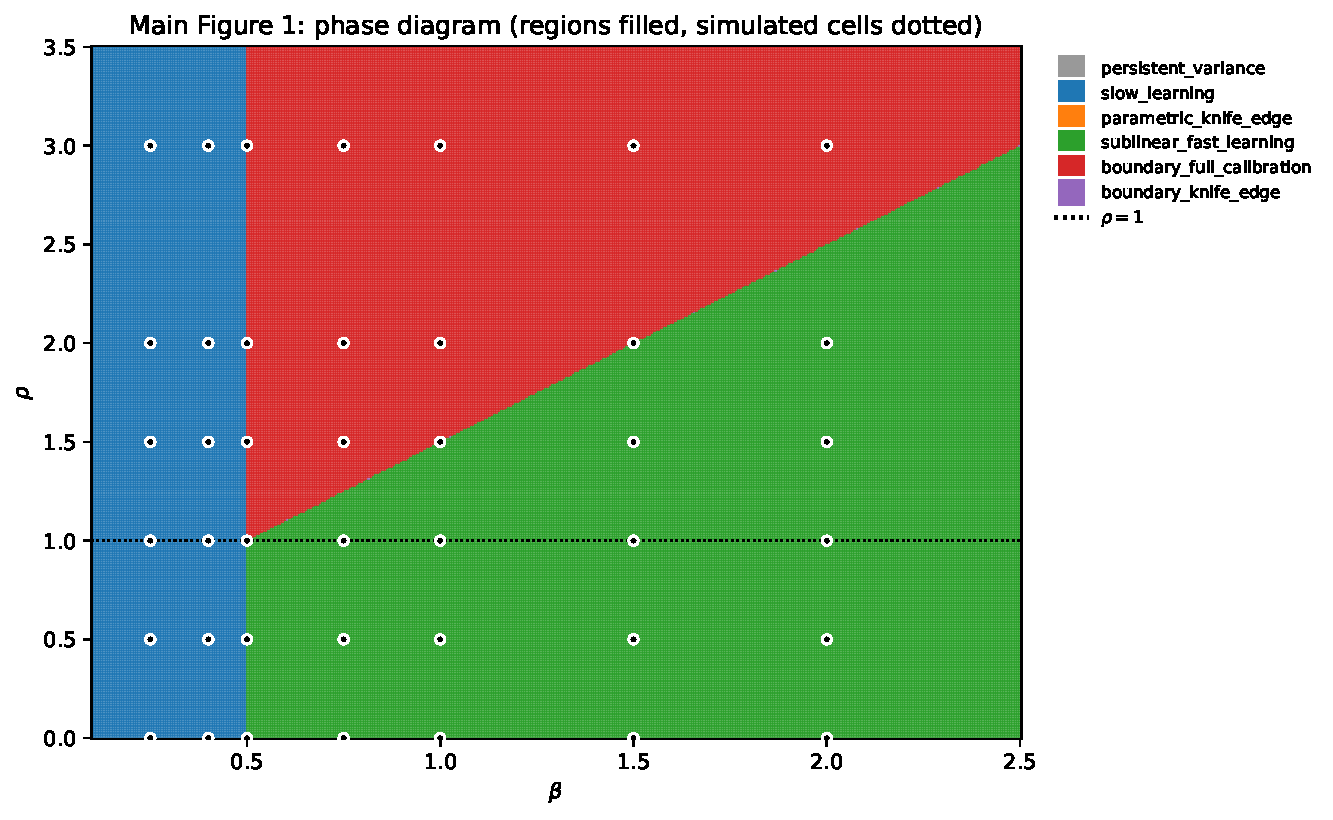
\includegraphics[width=0.7\linewidth]{figures/fig1_phase_diagram.pdf}
  \caption{Theoretical phase diagram in $(\beta,\rho)$ space. The five regimes of Theorem~\ref{thm:phase} partition the plane by the asymptotic behavior of the optimal calibration size $x_n^\star$. The horizontal line $\rho=1$ is the empirically common case in which the synthetic budget scales linearly with the real budget; the vertical line $\beta=1/2$ is the parametric knife edge. The labelled headline regime is the wide wedge $\beta>1/2$, $0<\rho<\beta+\tfrac12$, where the optimal calibration share vanishes despite the optimal calibration size diverging.}
  \label{fig:phase}
\end{figure}

% POLISHED


\section{Adaptive method and inference}
\label{sec:adaptive}

The oracle allocation $x_n^\star$ in Theorem~\ref{thm:phase} depends on unknown quantities: the real-estimator variance constant $a$, the synthetic-variance scale $v_n$, and the bias-curve constants $(c,\beta)$. \Cref{ssec:adaptive} gives a grid estimator that learns these quantities from pilot calibrations. \Cref{ssec:adaptive-oracle} shows that it tracks the oracle when the estimated risk curve is uniformly accurate in relative terms. \Cref{app:wald} (in the appendix, for space) then explains when the resulting point estimator supports ordinary Wald intervals.

\subsection{Adaptive grid-minimization estimator}\label{ssec:adaptive}

The idea is to estimate the profiled risk $R_n(x)$ on a discrete grid, choose the smallest estimated risk, and then apply the exact safety check $x\,B_n(x)<a$ from \Cref{prop:safe}. We use grid minimization rather than solving the first-order condition \cref{eq:foc} directly. The grid handles the boundary choices $x=0$ and $x=n$, avoids the smaller local maximum from \Cref{lem:critical}, and does not require estimating $\beta$ at a parametric rate.

% [Algorithm box (\Cref{alg:adaptive}) moved verbatim to \Cref{app:algbox}
%  to fit the 9-page main-content limit; the prose description below
%  references the full pseudocode in the appendix.]

\iffalse  %% original Algorithm 1 box -- now reproduced verbatim in Appendix
\begin{algorithm}[!t]
\caption{Corrected adaptive Generalized-Neyman estimator.}
\label{alg:adaptive}
\begin{algorithmic}[1]
\State \textbf{Input:} real sample $X_1,\dots,X_n$; calibratable generator $\mathcal{G}$; pilot grid $\mathcal{G}_{\mathrm{pilot}}$; full grid $\mathcal{G}_n^+:=\mathcal{G}_n\cup\{0,n\}$; number of folds $K$.
\State Cross-fit split $[n]$ into $K$ folds; for each fold, allocate out-of-fold data into calibration-pilot, validation, and final-estimation slices. Loop over folds.
\State Estimate $\hat a$ as the empirical variance of the influence-function values $\psi(X_i)$ on the out-of-fold slice.
\For{each $x_j\in\mathcal{G}_{\mathrm{pilot}}$}
  \State Calibrate $\mathcal{G}$ on $x_j$ pilot observations, draw $m_n$ synthetic points, compute $\hat\theta_S(x_j)$, and estimate $\hat v_n$ as the synthetic sample variance divided by $m_n$.
  \State Validation-debias the squared bias: $\widehat{b^2}(x_j)=\bigl[(\hat\theta_S(x_j)-\hat\theta_R^V)^2-\widehat{\mathrm{Var}}(\hat\theta_S(x_j))-\widehat{\mathrm{Var}}(\hat\theta_R^V)\bigr]_+$, where $\hat\theta_R^V$ is the real estimator on the validation slice.
\EndFor
\State Fit a power law by ordinary least squares: $\log\widehat{b^2}(x_j)=\log\hat c-2\hat\beta\log x_j+\epsilon_j$.
\State Form $\widehat{B}_n(x)=\hat v_n+\hat c\,x^{-2\hat\beta}$, $\widehat V_R(x)=\hat a/(n-x)$, and $\widehat R_n(x)=\widehat V_R(x)\widehat{B}_n(x)/[\widehat V_R(x)+\widehat{B}_n(x)]$ on $\mathcal{G}_n^+$, with $\widehat R_n(0)=\hat a/n$ and $\widehat R_n(n)=\widehat{B}_n(n)$.
\State $\hat x_n\gets \argmin_{x\in\mathcal{G}_n^+}\widehat R_n(x)$.
\State \textbf{Safety check:} if $\hat x_n\,\widehat{B}_n(\hat x_n)\ge\hat a$, return the all-real estimator $\hat\theta_R$.
\State Otherwise set $\hat\alpha=\widehat{B}_n(\hat x_n)/[\widehat V_R(\hat x_n)+\widehat{B}_n(\hat x_n)]$ and return $\hat\theta=\hat\alpha\,\hat\theta_R(\hat x_n)+(1-\hat\alpha)\,\hat\theta_S(\hat x_n)$.
\State \textbf{Output:} cross-fit average of $\hat\theta$ over the $K$ folds.
\end{algorithmic}
\end{algorithm}
\fi  %% end of moved Algorithm 1 box

The full pseudocode (\Cref{alg:adaptive} in \Cref{app:algbox}) uses the safe-improvement boundary from \Cref{prop:safe} directly. The same inequality that defines when synthetic augmentation can help also tells the procedure when to abstain. In step~6 of the pseudocode the squared bias is validation-debiased as $\widehat{b^2}(x_j)=\bigl[(\hat\theta_S(x_j)-\hat\theta_R^V)^2-\widehat{\mathrm{Var}}(\hat\theta_S(x_j))-\widehat{\mathrm{Var}}(\hat\theta_R^V)\bigr]_+$, and the truncation $[\,\cdot\,]_+$ prevents Monte~Carlo noise from producing negative squared-bias estimates; below we assume that this truncation is harmless on the part of the grid where variance dominates.

\subsection{Oracle inequality}\label{ssec:adaptive-oracle}

Grid minimization does not require $\widehat R_n$ to be accurate in absolute units. It only needs to rank grid points correctly with high probability. The right condition is uniform relative consistency.

\begin{theorem}[Adaptive oracle inequality]\label{thm:adaptive}
Let $\mathcal{G}_n^+:=\mathcal{G}_n\cup\{0,n\}$, $x_n^\star:=\argmin_{x\in\mathcal{G}_n^+}R_n(x)$, and $\hat x_n:=\argmin_{x\in\mathcal{G}_n^+}\widehat R_n(x)$. Suppose
\begin{equation}\label{eq:Delta-n}
  \Delta_n\;:=\;\sup_{x\in\mathcal{G}_n^+}\biggl|\frac{\widehat R_n(x)}{R_n(x)}-1\biggr|\;\stackrel{p}{\to}\;0.
\end{equation}
Then $R_n(\hat x_n)/R_n(x_n^\star)\stackrel{p}{\to}1$. If furthermore the grid satisfies $\inf_{x\in\mathcal{G}_n}R_n(x)/\inf_{x\in[0,n]}R_n(x)\to 1$, then $R_n(\hat x_n)/\inf_{x\in[0,n]}R_n(x)\stackrel{p}{\to}1$.
\end{theorem}

In words, the empirical risk curve only needs to be uniformly close to the true curve in \emph{ratio}. A constant multiplicative error in $\widehat R_n$ does not change the argmin, so the grid procedure can inherit the oracle rate even when the individual estimates of $a$, $v_n$, $c$, and $\beta$ converge slowly. This is why the grid version is preferable to a plug-in solver of the first-order condition, which would be more sensitive to slow convergence of $\hat\beta$.

% [Subsection ``Asymptotic distribution and Wald inference'' moved to
%  Appendix~\ref{app:wald} to fit the 9-page main-content limit. The
%  centered CLT (Proposition~\ref{prop:clt}), Wald-coverage corollary
%  (Corollary~\ref{cor:wald}), and discussion are reproduced there verbatim,
%  with proofs in \Cref{proof:clt,proof:wald}.]


% =====================================================================
% POLISHED


\section{Experiments}
\label{sec:experiments}

The experiments answer three questions. First, does the corrected oracle obey the phase diagram? Second, can an adaptive estimator recover useful allocations from finite pilot data? Third, when does the MSE-optimal estimator need validation debiasing for inference? Experiments~1, 2, and~4 use full synthetic Monte~Carlo sweeps; Experiments~1 and~2 together use roughly $10^7$ replications, and Experiment~4 uses $280{,}000$ replications. The multichannel, tabular, and causal benchmarks, together with complete result tables for all experiments, are reported in Appendix~\ref{app:experiments}.

\subsection{Phase-diagram validation}\label{ssec:exp1}

\paragraph{Setup.} Real observations follow $X_i=\theta^\star+\epsilon_i$ with $\epsilon_i\sim N(0,a)$. After calibration size $x$, synthetic observations follow $Z_j(x)=\theta^\star+B_0x^{-\beta}+u_j$ with $u_j\sim N(0,\sigma_S^2)$ and $m_n=\lceil \kappa n^\rho\rceil$. The main grid sets $\theta^\star=0$ and $a=B_0=c=\sigma_S^2=\kappa=1$, then sweeps $n\in\{100,\ldots,20{,}000\}$, seven values of $\beta\in[0.25,2]$, and six values of $\rho\in[0,3]$.

\paragraph{Main evidence.} The oracle results support the paper's main claim. In the headline cell ($\beta=1$, $\rho=1$, $n=20{,}000$), the corrected oracle has MSE ratio $0.535$ relative to all-real estimation. The old fixed-share rule has ratio $0.779$, and synthetic-only full calibration has ratio $1.015$. Thus the corrected allocation roughly doubles the MSE reduction obtained by the fixed-share rule, while synthetic-only use is slightly harmful. \Cref{fig:mse_compare} shows the same ordering across the grid. The scaling check in \Cref{fig:scaling} also matches the theory: among the interior fast-learning cells, the four disagreements are all upward deviations near the slow-learning boundary, consistent with finite-grid pre-asymptotics rather than a failure of the first-order condition. Full slope estimates are in \Cref{tab:scaling}.

\subsection{Adaptive feasibility}\label{ssec:exp2}

Experiment~2 uses the same Gaussian DGP on a smaller grid and estimates the bias curve from the pilot grid $\mathcal{G}_{\mathrm{pilot}}=\{5,10,20,40,80,160,320,640\}\cap[1,n/2]$. The adaptive story is more cautious than the oracle story. In the headline cell ($\beta=1$, $\rho=1$, $n=10{,}000$), the oracle MSE ratio is $0.522$, while \texttt{corrected\_adaptive\_gn} reaches $0.867$ and \texttt{safe\_corrected\_adaptive\_gn} reaches $0.908$. The selected calibration size is close to oracle in that cell ($563$ versus $573$), but the MSE gap shows that allocation tracking is not the same as oracle-equivalent point estimation.

Across the $60$ non-trivial cells with $\rho>0$, \texttt{corrected\_adaptive\_gn} is harmful in $21$ cells, with median MSE ratio $0.986$ and maximum ratio $1.460$. This is not evidence that the adaptive method has reached its asymptotic oracle regime at the simulated sample sizes. It is evidence for a more modest claim: the corrected risk curve and safety fallback make adaptive synthetic augmentation stable enough to avoid the much larger failures of naive synthetic-use rules. \Cref{fig:adaptive_alloc} and \Cref{fig:adaptive_regret} show allocation tracking and residual regret; full adaptive summaries are in \Cref{tab:adaptive}.

\subsection{Inference and coverage}\label{ssec:exp4}

Experiment~4 focuses on regimes where residual synthetic bias can be large relative to standard error: $\beta\in\{0.4,0.5,0.75,1.0\}$, $\rho=1$, and $n\in\{200,500,1000,2000,5000\}$. The point-estimation message and the inference message separate cleanly. Naive Wald intervals around the MSE-optimal estimator have the weakest coverage, with full-grid range $0.855$--$0.955$ and median $0.916$. Validation-debiased intervals have range $0.938$--$0.964$ and median $0.953$, closest to nominal among the synthetic intervals. The worst naive cell is the parametric knife edge ($\beta=0.5$, $\rho=1$, $n=500$), where naive coverage is $0.855$ and validation-debiased coverage is $0.954$. \Cref{fig:coverage} plots the full coverage curves, and \Cref{tab:coverage} gives the complete coverage summary.

\paragraph{Reproducibility.} Full configurations, raw and aggregated long-format results, and the analysis notebook used to render \Cref{fig:scaling}--\Cref{fig:coverage} are available at \texttt{<anon>} (URL withheld for blind submission).


% [Figures showing oracle scaling (\Cref{fig:scaling}) and MSE-ratio
%  comparison (\Cref{fig:mse_compare}) moved to Appendix~\ref{app:experiments}
%  to fit the 9-page main-content limit; reproduced there verbatim.]

% [Figures showing adaptive allocation/regret (\Cref{fig:adaptive_alloc},
%  \Cref{fig:adaptive_regret}) and 95\% interval coverage
%  (\Cref{fig:coverage}) moved to Appendix~\ref{app:experiments} to fit the
%  9-page main-content limit; full captions and panels are reproduced
%  there verbatim.]

% =====================================================================
% POLISHED


\section{Conclusion}
\label{sec:discussion}

Synthetic data do not eliminate the value of real data. They make real data more strategic. The paper's main message is that scarce real observations have two competing roles: they are evidence for the estimand and inputs that improve the synthetic generator. Treating calibration as a fixed-share preprocessing step misses this trade-off. The correct allocation is governed by marginal value: one more real observation should be spent on calibration only when the reduction in synthetic error is worth the loss of direct real-estimation precision.

This marginal-value logic changes the practical recommendation. In the central regime for modern synthetic-data pipelines, where synthetic samples scale with the real-data budget and generator bias declines quickly, the optimal calibration size grows but the calibration share vanishes. More synthetic scale does not mean spending a constant fraction of real data on calibration. It means using a growing, sublinear calibration set and preserving most real observations for direct estimation.

The same distinction matters for uncertainty quantification. MSE-optimal synthetic augmentation can improve point estimation while leaving residual bias large enough to damage naive confidence intervals. Valid inference therefore requires an explicit bias correction or an allocation rule designed for coverage rather than point risk. The broader lesson is simple: synthetic data are useful only when they are allocated, weighted, and debiased with the real-data budget in view.


\bibliographystyle{plainnat}
\bibliography{references}

\appendix

\section{Plateau bias}
\label{app:plateau}

\emph{This subsection was moved from the main paper (formerly Section~4.4) to fit the 9-page content limit; it is reproduced here verbatim.}

The phase diagram assumes the synthetic squared bias drives to zero with calibration. Foundation-model-style generators may instead leave a non-vanishing bias floor, such as alignment errors that more calibration data cannot remove. The next result records that, once such a floor is present, the regime structure collapses.

\begin{proposition}[Plateau-bias regime]\label{prop:plateau}
Replace Assumption~\ref{asm:pl} by $b_2(x)=b_\infty^2+cx^{-2\beta}\{1+o(1)\}$ with $b_\infty^2>0$ and $\beta>0$, and suppose Assumption~\ref{asm:vn} holds with $\rho\ge 0$. Then for $n$ sufficiently large the active interior root satisfies
\begin{equation}\label{eq:xn-plateau}
  x_n^\circ\;\le\;\Bigl(\tfrac{2\beta a c}{b_\infty^4}\Bigr)^{1/(2\beta+1)}\;=\;O(1),
\end{equation}
so $\lambda_n^\circ\to 0$ for every $\beta>0$ and every $\rho\ge 0$. The optimal risk satisfies $R_n(x_n^\star)=a/n\{1+o(1)\}$: synthetic augmentation buys at most a finite-sample shrinkage gain and no first-order rate improvement. The shrinkage is positive iff $x_n^\circ\,b_\infty^2<a$.
\end{proposition}

In words, plateau bias caps calibration at a constant budget regardless of how fast the bias \emph{would} have decayed before reaching the floor. Operationally, the generator is useful only down to its noise floor; beyond that point, further calibration is wasted.


\section{Asymptotic distribution and Wald inference}
\label{app:wald}

\emph{This subsection was moved from the main paper (formerly Section~5.3) to fit the 9-page content limit; it is reproduced here verbatim.}

A low-MSE point estimator does not automatically give a valid confidence interval. The same residual bias that the corrected oracle tolerates in mean square appears as an additive shift in the centered limit law. The next two results make that shift explicit.

\begin{proposition}[Centered asymptotic normality]\label{prop:clt}
Under Assumptions~\ref{asm:al-real},~\ref{asm:al-synth},~\ref{asm:pl}, and~\ref{asm:vn} with $v_n>0$ and a conditional Lindeberg condition on $\psi$ and $\phi_x$, the linear estimator at the oracle satisfies
\begin{equation}\label{eq:clt}
  \frac{\hat\theta^{\mathrm{L}}(\alpha^*(x_n^\star),x_n^\star)-\theta^*-(1-\alpha^*(x_n^\star))\,\Delta(x_n^\star)}{\sqrt{\Omega_n(x_n^\star)}}\;\Rightarrow\;N(0,1),
\end{equation}
conditionally on $\mathcal{F}_C$ and unconditionally, where $\Omega_n(x):=\alpha^*(x)^2 V_R(x)+(1-\alpha^*(x))^2 v_n$ is the stochastic-variance contribution and $\Delta(x):=\theta_x-\theta^*$ is the calibration-side bias. Replacing oracle quantities by their estimates from Theorem~\ref{thm:adaptive} preserves the CLT.
\end{proposition}

In plain English, the estimator is asymptotically normal around a shifted center, $\theta^*+(1-\alpha^*(x_n^\star))\,\Delta(x_n^\star)$, not necessarily around $\theta^*$. The shift is the synthetic weight times the remaining calibration bias. It matters for inference only when it is large relative to the standard error.

\begin{corollary}[Wald inference around $\theta^*$]\label{cor:wald}
A two-sided Wald interval centered at $\hat\theta^{\mathrm{L}}$ with width $z_{1-\alpha/2}\sqrt{\Omega_n(x_n^\star)}$ has asymptotic coverage $1-\alpha$ for $\theta^*$ if and only if
\begin{equation}\label{eq:wald-cond}
  (1-\alpha^*(x_n^\star))\,\Delta(x_n^\star)\;=\;o_p\bigl(\sqrt{\Omega_n(x_n^\star)}\bigr).
\end{equation}
Under Theorem~\ref{thm:phase}, in Regime~III with $\rho=1$ and $\beta>1/2$, condition Eq.~\ref{eq:wald-cond} holds; in Regime~V with $\rho=1$ and $\beta=1/2$ it generically fails.
\end{corollary}

In Regime~III, calibration is fast enough that $\Delta(x_n^\star)$ is of order $n^{-2\beta/(2\beta+1)}=o(n^{-1/2})$, smaller than the standard error $\sqrt{\Omega_n}\asymp n^{-1/2}$. Naive Wald intervals are therefore asymptotically valid in that regime, though finite samples can still show undercoverage. In the parametric knife-edge Regime~V, $\Delta(x_n^\star)$ and $\sqrt{\Omega_n}$ are the same order, and the shift in Eq.~\ref{eq:clt} produces undercoverage that does not vanish with $n$. In such cases, the validation-debiased construction of a PPI-type estimator subtracts an estimate of $\Delta(x_n^\star)$ using the held-out validation slice and restores nominal coverage at the cost of a constant-factor variance penalty.

% POLISHED


\section{Proofs of main results}
\label{app:proofs}

This appendix collects full proofs of the formal statements in the main paper. Throughout, we work in the linear-allocation configuration of \Cref{sec:setup}: the index set $[n] = \{1, \dots, n\}$ is partitioned into the calibration block $C_x$ of size $x$ and the estimation block $E_x = [n] \setminus C_x$ of size $n - x$, and we write $V_R(x) = a / (n-x)$ for the variance of the real-only estimator $\hat\theta_R$ on $E_x$ and $B_n(x) = v_n + c\, x^{-2\beta}$ for the effective synthetic-error variance. Assumptions~\ref{asm:al-real},~\ref{asm:al-synth},~\ref{asm:pl}, and~\ref{asm:vn} are in force throughout. The notation matches the main paper, including the convention $B_n(\cdot)$ for the effective synthetic-error variance.

\subsection{Auxiliary lemmas}\label{ssec:aux}

We use two auxiliary lemmas repeatedly. Both follow from sample splitting and the working model and are standard.

\begin{lemma}[Conditional and unconditional independence]
\label{lem:ci} Fix $x$ and suppose the split $(C_x,E_x)$ is  independent of $\{X_i\}_{i=1}^n$. Assume that, conditionally on $\mathcal F_C$, the synthetic observations $Z_1,\ldots,Z_{m_n}$ are generated from an auxiliary random stream independent of $\{X_i:i\in E_x\}$. Then:
\[
\hat\theta_R(E_x)\perp\!\!\!\perp \hat\theta_S(x)\mid \mathcal F_C.
\]
Moreover,
\[
\hat\theta_R(E_x)\perp\!\!\!\perp (\theta_x,\hat\theta_S(x)).
\]
Consequently, $\hat\theta_R(E_x)$ is independent of both $\hat\theta_S(x)-\theta_x$ and $\hat\theta_S(x)-\theta^*$.
\end{lemma}

\begin{proof}
Because the split is independent of the data and the observations are i.i.d., the estimation sample $\{X_i:i\in E_x\}$ is independent of $\mathcal F_C$. Conditional on $\mathcal F_C$, the calibrated distribution $P_x$ and the pseudo-true parameter $\theta_x=\theta(P_x)$ are fixed, and the synthetic sample $Z_1,\ldots,Z_{m_n}$ is generated using an auxiliary random stream independent of the estimation sample. Hence $\hat\theta_R(E_x)$ and $\hat\theta_S(x)$ are conditionally independent given $\mathcal F_C$.

For the unconditional statement, $\hat\theta_R(E_x)$ is measurable with respect to the estimation sample, while $(\theta_x,\hat\theta_S(x))$ is measurable with respect to the calibration sample together with the auxiliary synthetic stream. These two sources of randomness are independent. Therefore
\[
\hat\theta_R(E_x)\perp\!\!\!\perp (\theta_x,\hat\theta_S(x)).
\]
The two displayed consequences follow because $\hat\theta_S(x)-\theta_x$ and $\hat\theta_S(x)-\theta^*$ are measurable functions of $(\theta_x,\hat\theta_S(x))$.
\end{proof}

\begin{lemma}[Synthetic-error decomposition]\label{lem:Bn}
Under Assumption~\ref{asm:al-synth} and~\ref{asm:pl}, the synthetic estimator's mean-squared error around $\theta^\star$ admits the decomposition
\[
\mathbb{E}\bigl[(\hat\theta_S(x) - \theta^\star)^2\bigr]
= v_n + b_2(x) + o(v_n) + o(b_2(x))
= B_n(x) \{1 + o(1)\},
\]
where $b(x) := \theta_x - \theta^\star$ is the calibration-induced bias and $B_n(x) := v_n + c\,x^{-2\beta}$.
\end{lemma}

\begin{proof}[Proof of \Cref{lem:Bn}]
Decompose $\hat\theta_S(x) - \theta^\star = (\hat\theta_S(x) - \theta_x) + b(x)$. By Assumption~\ref{asm:al-synth}, the first term has conditional mean zero and conditional variance $\sigma_S^2/m_n + o_p(1/m_n) = v_n\{1+o(1)\}$ (using $v_n = \sigma_S^2/m_n$ from the working model). Squaring and taking the unconditional expectation, the cross term vanishes (mean-zero conditional on the calibration data, applied with the tower property), and the squared bias term equals $b_2(x) = c x^{-2\beta}\{1+o(1)\}$ by Assumption~\ref{asm:pl}. Combining gives the displayed decomposition.
\end{proof}



\subsection{Proof of \texorpdfstring{\Cref{lem:mse-decomp}}{Lemma~\ref{lem:mse-decomp}} (Working MSE)}\label{proof:mse-decomp}

\begin{proof}[Proof of \Cref{lem:mse-decomp}]
Fix $x$ in the calibration range under consideration and write $\xi_R:=\hat\theta_R(E_x)-\theta^\star$ and $\xi_S:=\hat\theta_S(x)-\theta^\star$. Then $\hat\theta^L(\alpha,x)-\theta^\star=\alpha\xi_R+(1-\alpha)\xi_S$. By the unconditional independence statement in Lemma~\ref{lem:ci}, $\xi_R$ and $\xi_S$ are independent. Hence
\[
\mathbb{E}\left[\{\alpha\xi_R+(1-\alpha)\xi_S\}^2\right]
=
\alpha^2\mathbb{E}[\xi_R^2]
+
(1-\alpha)^2\mathbb{E}[\xi_S^2]
+
2\alpha(1-\alpha)\mathbb{E}[\xi_R]\mathbb{E}[\xi_S].
\]
By Assumption~\ref{asm:al-real}, the real estimator has a mean-zero influence function and a mean-zero remainder, so $\mathbb{E}[\xi_R]=0$. Thus the cross term vanishes exactly. Moreover, Assumption~\ref{asm:al-real} gives $\mathbb{E}[\xi_R^2] = V_R(x)\{1+o(1)\}$, uniformly over the calibration range. By \Cref{lem:Bn}, the synthetic-error decomposition gives $\mathbb{E}[\xi_S^2] = B_n(x)\{1+o(1)\}$, uniformly over the same range. Substituting these two expansions into the preceding display yields
\[
\mathbb{E}\bigl[(\hat\theta^L(\alpha,x)-\theta^\star)^2\bigr]
=
\alpha^2V_R(x)+(1-\alpha)^2B_n(x)+\mathcal R_n(\alpha,x),
\]
where $\mathcal R_n(\alpha,x)=\alpha^2o\{V_R(x)\}+(1-\alpha)^2o\{B_n(x)\}$. Since $\alpha\in[0,1]$, both $\alpha^2$ and $(1-\alpha)^2$ are bounded by one, and therefore $\mathcal R_n(\alpha,x)=o\{V_R(x)\}+o\{B_n(x)\}$ uniformly in $\alpha\in[0,1]$. This proves the claim.
\end{proof}

\subsection{Proof of \texorpdfstring{\Cref{prop:mix}}{Proposition~\ref{prop:mix}} (Optimal mixing)}\label{proof:mix}

\begin{proof}[Proof of \Cref{prop:mix}]
Define the leading-order MSE
\[
\overline{\mathrm{MSE}}_n(\alpha, x) := \alpha^2 V_R(x) + (1-\alpha)^2 B_n(x).
\]
This is a quadratic function of $\alpha$. Its second derivative with respect to $\alpha$ is $2[V_R(x) + B_n(x)] > 0$ since both terms are strictly positive, so $\overline{\mathrm{MSE}}_n(\cdot, x)$ is strictly convex. Setting the first derivative to zero gives
\[
\frac{\partial}{\partial \alpha}\, \overline{\mathrm{MSE}}_n(\alpha, x)
= 2\alpha V_R(x) - 2(1-\alpha) B_n(x) = 0,
\]
which solves to $\alpha^\star(x) = B_n(x) / [V_R(x) + B_n(x)] \in (0,1)$ since both $V_R(x)$ and $B_n(x)$ are strictly positive and finite. This is the unique unconstrained minimizer; because it lies in the open interval $(0,1)$, it is also the unique minimizer over $[0,1]$.

Substituting $\alpha = \alpha^\star(x)$ back into $\overline{\mathrm{MSE}}_n$ and simplifying,
\[
R_n(x) := \overline{\mathrm{MSE}}_n(\alpha^\star(x), x)
= \frac{B_n(x)^2}{[V_R(x)+B_n(x)]^2} V_R(x)
+ \frac{V_R(x)^2}{[V_R(x)+B_n(x)]^2} B_n(x)
= \frac{V_R(x) B_n(x)}{V_R(x) + B_n(x)},
\]
which is the harmonic-mean form. Multiplying numerator and denominator by $(n-x)$ and using $V_R(x) = a/(n-x)$ gives the second equality
\[
R_n(x) = \frac{a\, B_n(x)}{a + (n-x)\, B_n(x)}. \qedhere
\]
\end{proof}


\subsection{Proof of \texorpdfstring{\Cref{prop:foc}}{Proposition~\ref{prop:foc}} (Exact FOC)}\label{proof:foc}

To prove \Cref{prop:foc} we first record an intermediate result on the gradient of the profiled risk. This auxiliary lemma is local to the appendix.

Define
\begin{equation}\label{eq:Phi-def-app}
\Phi(x) := B_n(x)^2\, x^{2\beta+1}, \qquad x > 0,
\end{equation}
and
\begin{equation}\label{eq:H-def-app}
H(x) := a\, B_n'(x) + B_n(x)^2.
\end{equation}

\begin{lemma}[Gradient of the profiled risk]\label{lem:gradient}
For every $x \in (0, n)$,
\begin{equation}\label{eq:Rn-prime-app}
R_n'(x) = \frac{a\, H(x)}{[a + (n-x)\, B_n(x)]^2}
       = \frac{a}{[a + (n-x) B_n(x)]^2}
        \cdot \frac{\Phi(x) - 2\beta a c}{x^{2\beta+1}}.
\end{equation}
In particular, $\mathrm{sign}(R_n'(x)) = \mathrm{sign}(\Phi(x) - 2\beta a c)$.
\end{lemma}
\begin{proof}
Write $R_n = u/w$ with $u(x) = a\, B_n(x)$ and $w(x) = a + (n-x)\, B_n(x)$. Differentiating,
\[
u'(x) = a\, B_n'(x), \qquad
w'(x) = -B_n(x) + (n-x)\, B_n'(x).
\]
By the quotient rule, $R_n'(x) = (u'w - u w') / w^2$. Compute the numerator:
\begin{align*}
u' w - u w'
&= a B_n' \bigl[a + (n-x) B_n\bigr]
   - a B_n \bigl[-B_n + (n-x) B_n'\bigr] \\
&= a^2 B_n' + a(n-x) B_n B_n' + a B_n^2 - a(n-x) B_n B_n' \\
&= a^2 B_n' + a B_n^2 = a\, H(x).
\end{align*}
The two cross terms $\pm a(n-x) B_n B_n'$ cancel exactly; this algebraic cancellation is the reason the optimum does not depend on $n - x$ at first order.

To rewrite in terms of $\Phi$, substitute $B_n'(x) = -2\beta c\, x^{-(2\beta+1)}$ (from $B_n(x) = v_n + c x^{-2\beta}$) and multiply $H(x)$ by $x^{2\beta+1}$:
\[
H(x)\, x^{2\beta+1}
= -2\beta a c + B_n(x)^2 x^{2\beta+1}
= \Phi(x) - 2\beta a c.
\]
Dividing by $x^{2\beta+1}$ and substituting into $R_n'(x) = a H(x)/w^2$ gives the second equality in \cref{eq:Rn-prime-app}. The denominator $[a + (n-x) B_n(x)]^2$ is strictly positive on $(0,n)$, and $a$ and $x^{2\beta+1}$ are strictly positive, so $R_n'(x)$ has the same sign as $\Phi(x) - 2\beta a c$.
\end{proof}

\begin{proof}[Proof of \Cref{prop:foc}]
By \Cref{lem:gradient}, the interior critical points of $R_n$ on $(0,n)$ are exactly the points where $H(x) = 0$, equivalently $\Phi(x) = 2\beta a c$. Writing $\Phi(x) = (v_n + c x^{-2\beta})^2 x^{2\beta+1}$ and dividing both sides of $\Phi(x) = 2\beta a c$ by $x^{2\beta+1}$ gives the FOC
\[
(v_n + c x^{-2\beta})^2 = 2\beta a c\, x^{-(2\beta+1)},
\]
which is \cref{eq:foc} of the main paper. Multiplying by $x^{2\beta+1}$ and expanding the square,
\[
(v_n + c x^{-2\beta})^2 x^{2\beta+1}
= v_n^2 x^{2\beta+1} + 2 v_n c x + c^2 x^{1-2\beta},
\]
so the polynomial form
\[
v_n^2 x^{2\beta+1} + 2 v_n c\, x + c^2 x^{1-2\beta} = 2\beta a c
\]
is equivalent. The multiplicity claim follows from the critical-point structure (see \Cref{proof:critical} below): for $\beta \le 1/2$, $\Phi$ is strictly increasing, so $\Phi(x) = 2\beta a c$ has at most one solution; for $\beta > 1/2$, $\Phi$ is strictly U-shaped with minimum at $x^\dagger$, so $\Phi(x) = 2\beta a c$ has at most two solutions, and the active interior root (the local minimum of $R_n$) is the larger.
\end{proof}

\subsection{Proof of \texorpdfstring{\Cref{prop:safe}}{Proposition~\ref{prop:safe}} (Safe-improvement)}\label{proof:safe}

\begin{proof}[Proof of \Cref{prop:safe}]
The all-real benchmark uses every real observation for direct estimation, incurring risk $a/n$. We compare $R_n(x)$ with $a/n$ via direct algebra. By \Cref{prop:mix},
\[
R_n(x) = \frac{a\, B_n(x)}{a + (n-x)\, B_n(x)}.
\]
Then $R_n(x) < a/n$ iff $a\, B_n(x) \cdot n < a \cdot [a + (n-x) B_n(x)]$, i.e.\ iff $n B_n(x) < a + (n-x) B_n(x)$, which simplifies after subtracting $(n-x) B_n(x)$ from both sides to
\[
x\, B_n(x) < a.
\]
The boundary case is $R_n(0) = a B_n(0)/(a + n B_n(0)) \le a/n$ trivially (with equality only in the degenerate $B_n(0) = \infty$ limit); the restriction to $x \in (0, n)$ is what makes the iff statement non-trivial. Substituting $B_n(x) = v_n + c x^{-2\beta}$ gives the equivalent form $x(v_n + c x^{-2\beta}) < a$, i.e.\ $v_n x + c x^{1-2\beta} < a$.
\end{proof}

\subsection{Proof of \texorpdfstring{\Cref{lem:critical}}{Lemma~\ref{lem:critical}} (Critical points)}\label{proof:critical}

We first establish the shape of $\Phi$ as an auxiliary lemma, then conclude about critical points of $R_n$.

\begin{lemma}[Shape of $\Phi$]\label{lem:shape}
Under Assumption~\ref{asm:pl}, the function $\Phi(x) = (v_n + c x^{-2\beta})^2 x^{2\beta+1}$ on $(0,\infty)$ satisfies:
\begin{enumerate}[label=\rm(\alph*),leftmargin=*]
\item $\Phi'(x) = x^{2\beta} B_n(x) [(2\beta+1) v_n + (1-2\beta) c x^{-2\beta}]$.
\item If $\beta \le 1/2$, then $\Phi'(x) > 0$ for all $x > 0$ (with $v_n > 0$): $\Phi$ is strictly increasing, with $\Phi(0^+) = c^2 \mathbf{1}\{\beta = 1/2\}$ and $\Phi(\infty) = +\infty$.
\item If $\beta > 1/2$, then $\Phi$ is strictly U-shaped on $(0,\infty)$ with unique minimum at
\begin{equation}\label{eq:xdagger-app}
x^\dagger = \biggl(\frac{c(2\beta-1)}{(2\beta+1)v_n}\biggr)^{1/(2\beta)},
\end{equation}
and minimum value
\begin{equation}\label{eq:Phidagger-app}
\Phi^\dagger := \Phi(x^\dagger)
= K(\beta)\, c^{(2\beta+1)/(2\beta)}\, v_n^{(2\beta-1)/(2\beta)},
\quad
K(\beta) := \frac{16 \beta^2}{(2\beta+1)^{(2\beta+1)/(2\beta)}\,
                              (2\beta-1)^{(2\beta-1)/(2\beta)}}.
\end{equation}
$\Phi(0^+) = \Phi(\infty) = +\infty$.
\end{enumerate}
\end{lemma}

\begin{proof}[Proof of \Cref{lem:shape}]
\textbf{(a)} By the product rule applied to $\Phi(x) = B_n(x)^2 \cdot x^{2\beta+1}$,
\begin{align*}
\Phi'(x)
&= 2 B_n(x) B_n'(x) x^{2\beta+1} + B_n(x)^2 (2\beta+1) x^{2\beta} \\
&= x^{2\beta} B_n(x)\, \bigl[2 B_n'(x)\, x + (2\beta+1) B_n(x)\bigr].
\end{align*}
Substituting $B_n'(x) = -2\beta c x^{-(2\beta+1)}$ and $B_n(x) = v_n + c x^{-2\beta}$,
\begin{align*}
2 B_n'(x) x + (2\beta+1) B_n(x)
&= -4\beta c x^{-2\beta} + (2\beta+1) v_n + (2\beta+1) c x^{-2\beta} \\
&= (2\beta+1) v_n + (1 - 2\beta) c x^{-2\beta}.
\end{align*}
This proves (a).

\textbf{(b)} For $\beta \le 1/2$ we have $1 - 2\beta \ge 0$ and $v_n > 0$, so the bracket $(2\beta+1) v_n + (1-2\beta) c x^{-2\beta}$ is strictly positive on $(0,\infty)$. Combined with $x^{2\beta} > 0$ and $B_n(x) > 0$, this gives $\Phi'(x) > 0$ everywhere; $\Phi$ is strictly increasing. The endpoint behavior follows from expanding $B_n$. As $x \to 0^+$, $B_n(x) \sim c x^{-2\beta}$ so $\Phi(x) \sim c^2 x^{1 - 2\beta}$; for $\beta < 1/2$ this tends to $0$, while for $\beta = 1/2$, $\Phi(x) = (v_n x + c)^2 \to c^2$. As $x \to \infty$, $B_n(x) \to v_n$ so $\Phi(x) \sim v_n^2 x^{2\beta+1} \to \infty$ since $v_n > 0$.

\textbf{(c)} For $\beta > 1/2$, $1 - 2\beta < 0$. The bracket $(2\beta+1) v_n + (1-2\beta) c x^{-2\beta}$ is a strictly increasing function of $x$ (since $c x^{-2\beta}$ is strictly decreasing in $x$ and is multiplied by a negative coefficient). It vanishes when $c x^{-2\beta} = (2\beta+1) v_n / (2\beta - 1)$, equivalently at $x = x^\dagger$ given by \cref{eq:xdagger-app}. For $x < x^\dagger$ the bracket is negative, so $\Phi' < 0$; for $x > x^\dagger$ the bracket is positive, so $\Phi' > 0$. Hence $\Phi$ is strictly decreasing on $(0, x^\dagger)$ and strictly increasing on $(x^\dagger, \infty)$, with unique minimum at $x^\dagger$.

To compute $\Phi^\dagger = \Phi(x^\dagger)$, use $c x^{\dagger\, -2\beta} = (2\beta+1) v_n / (2\beta-1)$, so
\[
B_n(x^\dagger) = v_n + \frac{(2\beta+1) v_n}{2\beta - 1}
= v_n \cdot \frac{4\beta}{2\beta - 1}.
\]
From \cref{eq:xdagger-app}, $x^{\dagger\, 2\beta+1} = [c(2\beta-1) / ((2\beta+1) v_n)]^{(2\beta+1)/(2\beta)}$. Multiplying,
\begin{align*}
\Phi^\dagger
&= \Bigl(\tfrac{4\beta v_n}{2\beta - 1}\Bigr)^2
   \cdot \Bigl(\tfrac{c(2\beta-1)}{(2\beta+1) v_n}\Bigr)^{(2\beta+1)/(2\beta)} \\
&= \frac{16 \beta^2\, c^{(2\beta+1)/(2\beta)}}{(2\beta+1)^{(2\beta+1)/(2\beta)}
   (2\beta-1)^{(2\beta-1)/(2\beta)}}
   \cdot v_n^{(2\beta-1)/(2\beta)},
\end{align*}
where the $v_n$ exponent is $2 - (2\beta+1)/(2\beta) = (2\beta-1)/(2\beta)$ and the $(2\beta-1)$ exponent is $(2\beta+1)/(2\beta) - 2 = (1-2\beta)/(2\beta)$, contributing the factor $(2\beta-1)^{-(2\beta-1)/(2\beta)}$ as displayed. Endpoint behavior: as $x \to 0^+$, $\Phi(x) \sim c^2 x^{1-2\beta} \to +\infty$ since $1-2\beta < 0$; as $x \to \infty$, $\Phi(x) \sim v_n^2 x^{2\beta+1} \to +\infty$.
\end{proof}

\begin{proof}[Proof of \Cref{lem:critical}]
By \Cref{lem:gradient}, the interior critical points of $R_n$ on $(0,n)$ are exactly the points where $\Phi(x) = 2\beta a c$, and $\mathrm{sign}(R_n'(x)) = \mathrm{sign}(\Phi(x) - 2\beta a c)$.

\textbf{(i) $\beta \le 1/2$.} By \Cref{lem:shape}(b), $\Phi$ is strictly increasing, so the level set $\{x : \Phi(x) = 2\beta a c\}$ contains at most one element. When it exists, call it $x^\circ$. Then $\Phi - 2\beta a c < 0$ on $(0, x^\circ)$ and $> 0$ on $(x^\circ, \infty)$, so $R_n' < 0$ before $x^\circ$ and $R_n' > 0$ after; thus $x^\circ$ is a strict local minimum.

For $\beta < 1/2$, \Cref{lem:shape}(b) gives $\Phi(0^+) = 0 < 2\beta a c < \Phi(\infty) = \infty$, so $x^\circ$ exists by continuity. For $\beta = 1/2$, $\Phi(0^+) = c^2$ and $\Phi(\infty) = \infty$, so $x^\circ$ exists iff $c^2 < 2\beta a c = a c$, equivalently $c < a$.

\textbf{(ii) $\beta > 1/2$.} By \Cref{lem:shape}(c), $\Phi$ is U-shaped on $(0,\infty)$ with minimum value $\Phi^\dagger$ attained at $x^\dagger$.

\emph{Case (a)} If $\Phi^\dagger > 2\beta a c$, then $\Phi(x) > \Phi^\dagger > 2\beta a c$ for all $x > 0$, so $R_n' > 0$ throughout $(0,n)$ and there is no interior critical point.

\emph{Case (b)} If $\Phi^\dagger = 2\beta a c$, $\Phi - 2\beta a c \ge 0$ with equality only at $x^\dagger$, so $R_n' \ge 0$ with $R_n'(x^\dagger) = 0$; $R_n'$ does not change sign, so $x^\dagger$ is an inflection point but not a strict local extremum.

\emph{Case (c)} If $\Phi^\dagger < 2\beta a c$: since $\Phi(0^+) = \Phi(\infty) = +\infty$ and $\Phi$ is continuous and strictly U-shaped with minimum $\Phi^\dagger < 2\beta a c$, the equation $\Phi(x) = 2\beta a c$ has exactly two solutions $x_1 \in (0, x^\dagger)$ and $x_2 \in (x^\dagger, \infty)$ by the intermediate value theorem applied to each strictly monotone branch. On $(0, x_1)$, $\Phi > 2\beta a c$ so $R_n' > 0$; on $(x_1, x_2)$, $\Phi < 2\beta a c$ so $R_n' < 0$; on $(x_2, \infty)$, $\Phi > 2\beta a c$ so $R_n' > 0$. Hence $x_1$ is a strict local maximum and $x_2$ a strict local minimum of $R_n$.

The asymptotic claim follows from \cref{eq:Phidagger-app} and Assumption~\ref{asm:vn}: with $v_n = v_0 n^{-\rho}\{1 + o(1)\}$,
\[
\Phi^\dagger = K(\beta)\, c^{(2\beta+1)/(2\beta)}\, v_0^{(2\beta-1)/(2\beta)}\,
n^{-\rho(2\beta-1)/(2\beta)}\{1 + o(1)\},
\]
which tends to $0$ when $\rho > 0$ and $\beta > 1/2$, since the exponent $-\rho(2\beta-1)/(2\beta)$ is strictly negative. Hence $\Phi^\dagger < 2\beta a c$ for all sufficiently large $n$, putting us in case (iic).
\end{proof}

\subsection{Proof of \texorpdfstring{Theorem~\ref{thm:phase}}{Theorem~\ref{thm:phase}} (Phase diagram)}\label{proof:phase}

\begin{proof}[Proof of Theorem~\ref{thm:phase}]
We analyze the polynomial form of the FOC,
\begin{equation}\label{eq:foc-poly-app}
v_n^2 x^{2\beta+1} + 2 c v_n\, x + c^2 x^{1-2\beta} = 2 \beta a c,
\end{equation}
in each regime, using \Cref{lem:critical} for existence and identification of the active root, and the global minimization $x_n^\star \in \argmin_{x \in [0,n]} R_n(x)$.

\medskip
\noindent\textbf{Regime I ($\rho = 0$, $v_n \to v_0 > 0$).} With $v_n \to v_0$, the FOC \cref{eq:foc-poly-app} reads $v_0^2 x^{2\beta+1} + 2 c v_0\, x + c^2 x^{1-2\beta} = 2\beta a c + o(1)$, which has no $n$-dependence in the leading coefficients. By \Cref{lem:critical}, any active interior root is determined by the constants $(a, c, v_0, \beta)$ alone and is therefore $O(1)$. Since the budget $n$ grows unboundedly, $x_n^\circ / n \to 0$. The candidates $\{0, x_n^\circ, n\}$ are evaluated by direct substitution into $R_n$; the global minimizer is one of $\{0, x_n^\circ\}$ since $R_n(n) = v_n + c n^{-2\beta} \to v_0$ does not vanish, while $R_n(0) = a/n \to 0$. Hence $x_n^\star \in \{0, x_n^\circ\}$ and in either case $\lambda_n^\star = x_n^\star / n \to 0$.

\medskip
\noindent\textbf{Regime II ($\beta < 1/2$, $\rho > 0$).} Now $v_n \to 0$. We claim $x_n^\circ = \Theta(1)$. With $x$ bounded, $v_n^2 x^{2\beta+1} = O(v_n^2)$ and $2 c v_n x = O(v_n)$, both $o(1)$, so \cref{eq:foc-poly-app} reduces to $c^2 x^{1-2\beta} = 2\beta a c + o(1)$. Solving, $x^{1-2\beta} = 2\beta a / c + o(1)$, so $x_n^\circ \to x_\infty := (2\beta a / c)^{1/(1-2\beta)}$. To rule out the alternative $x_n^\circ \to \infty$, observe that if so, then because $1 - 2\beta > 0$, the term $c^2 x^{1-2\beta} \to \infty$, contradicting \cref{eq:foc-poly-app} (whose right side is finite). So indeed $x_n^\circ = \Theta(1)$, hence $x_n^\circ / n \to 0$.

For the rate: $V_R(x_n^\circ) = a/(n - x_n^\circ) \sim a/n$ since $x_n^\circ = O(1) \ll n$. And $B_n(x_n^\circ) = v_n + c x_n^{\circ\, -2\beta} \to c x_\infty^{-2\beta} > 0$ (the $v_n$ term vanishes). Substituting into the harmonic-mean form of $R_n$,
\[
R_n(x_n^\circ) = \frac{V_R B_n}{V_R + B_n}
= V_R \cdot \frac{1}{1 + V_R / B_n}
= V_R - \frac{V_R^2}{B_n} + O\bigl((V_R/B_n)^3\bigr),
\]
which yields $R_n(x_n^\circ) = a/n - (a/n)^2 / (c x_\infty^{-2\beta}) + o(n^{-2})$ as displayed in the theorem. Safe-improvement:
\[
x_\infty B_n(x_\infty) \to x_\infty \cdot c x_\infty^{-2\beta}
= c x_\infty^{1 - 2\beta} = c \cdot (2\beta a / c) = 2\beta a < a
\]
since $\beta < 1/2$. Hence by \Cref{prop:safe}, $R_n(x_n^\circ) < a/n$ for $n$ large, and the global oracle is $x_n^\star = x_n^\circ\{1+o(1)\}$.

\medskip
\noindent\textbf{Regime III ($\beta > 1/2$, $0 < \rho < \beta + 1/2$).} By \Cref{lem:critical}(iic), the active interior root $x_n^\circ$ exists for all $n$ sufficiently large. We make and verify the conjecture that the bias term is asymptotically negligible relative to the synthetic-variance term at the root: $c x_n^{\circ\, -2\beta} \ll v_n$, hence $B_n(x_n^\circ) = v_n\{1 + o(1)\}$. Substituting this into the FOC \cref{eq:foc} gives
\[
v_n^2 = 2\beta a c\, x_n^{\circ\, -(2\beta+1)}\{1+o(1)\},
\]
which solves to
\begin{align*}
x_n^\circ
&= \Bigl(\tfrac{2\beta a c}{v_n^2}\Bigr)^{1/(2\beta+1)}\{1+o(1)\} \\
&= \Bigl(\tfrac{2\beta a c}{v_0^2}\Bigr)^{1/(2\beta+1)}
   n^{2\rho/(2\beta+1)}\{1+o(1)\},
\end{align*}
using $v_n = v_0 n^{-\rho}\{1+o(1)\}$ to substitute. This is the displayed expression \cref{eq:xn-circ-III}.

To verify the conjecture, compute the ratio of the two terms in $B_n$:
\begin{align*}
\frac{c x_n^{\circ\, -2\beta}}{v_n}
&= c \cdot \Bigl[\tfrac{2\beta a c}{v_0^2}\Bigr]^{-2\beta/(2\beta+1)}
   n^{-4\beta\rho/(2\beta+1)} \cdot \frac{1}{v_0 n^{-\rho}}\{1+o(1)\} \\
&\asymp n^{-4\beta\rho/(2\beta+1) + \rho}
= n^{\rho \cdot \bigl[1 - 4\beta/(2\beta+1)\bigr]}
= n^{-\rho(2\beta-1)/(2\beta+1)},
\end{align*}
which tends to $0$ as $n \to \infty$ since $\beta > 1/2$ and $\rho > 0$. Hence $c x_n^{\circ\, -2\beta} = o(v_n)$, confirming the conjecture.

Feasibility: $x_n^\circ / n \asymp n^{2\rho/(2\beta+1) - 1}$. The exponent $2\rho/(2\beta+1) - 1$ is strictly negative iff $\rho < \beta + 1/2$, which is the assumed range. Hence $x_n^\circ = o(n)$, so $\lambda_n^\circ \to 0$.

Safe-improvement: $x_n^\circ B_n(x_n^\circ) \asymp n^{2\rho/(2\beta+1)} \cdot n^{-\rho} = n^{-\rho(2\beta-1)/(2\beta+1)} \to 0 < a$, so by \Cref{prop:safe}, $R_n(x_n^\circ) < a/n$ for $n$ large. We also have $R_n(x_n^\circ) < R_n(n)$ in this regime by Regime~IV's analysis below (strict inequality at the boundary). Hence $x_n^\star = x_n^\circ\{1+o(1)\}$.

For the risk asymptotics: $V_R(x_n^\circ) = a/(n - x_n^\circ) = a/n\{1+o(1)\}$ since $x_n^\circ = o(n)$, and $B_n(x_n^\circ) = v_n\{1+o(1)\}$. The harmonic-mean formula
\[
R_n(x_n^\star) = \frac{V_R B_n}{V_R + B_n}\{1+o(1)\}
              = \frac{(a/n)\, v_n}{a/n + v_n}\{1+o(1)\}
\]
yields the three subcases by direct substitution: if $\rho < 1$, $v_n \gg a/n$ so the denominator is dominated by $v_n$ and $R_n \sim a/n$; if $\rho = 1$, both terms are of the same order $1/n$ and $R_n \sim a v_0 / [(a + v_0) n]$; if $\rho > 1$, $v_n \ll a/n$ so the denominator is dominated by $a/n$ and $R_n \sim v_n = v_0/n^\rho$.

\medskip
\noindent\textbf{Regime IV ($\beta > 1/2$, $\rho > \beta + 1/2$).} The Regime-III asymptotic formula gives $x_n^\circ \asymp n^{2\rho/(2\beta+1)}$. Here $2\rho/(2\beta+1) > 1$, so $x_n^\circ > n$ for $n$ large and the interior root is infeasible. We compare the boundary candidates $R_n(0) = a/n$ and $R_n(n) = v_n + c n^{-2\beta}$. With $\rho > \beta + 1/2 > 1$ and $2\beta > 1$, $v_n = O(n^{-\rho}) = o(n^{-1})$ and $c n^{-2\beta} = o(n^{-1})$, so $R_n(n) = o(n^{-1}) < a/n$ eventually. Hence the global oracle is at the right boundary: $x_n^\star = n\{1+o(1)\}$, $\lambda_n^\star \to 1$, and the risk rate $R_n(x_n^\star) = v_n + c n^{-2\beta} = o(n^{-1})$ beats the all-real rate.

\medskip
\noindent\textbf{Regime V ($\beta = 1/2$).} With $\beta = 1/2$, the FOC \cref{eq:foc} becomes $(v_n + c x^{-1})^2 = a c x^{-2}$, i.e., $(v_n x + c)^2 = a c$ after multiplying through by $x^2$. Taking the positive square root (the negative root $v_n x + c = -\sqrt{a c}$ gives $x < 0$, infeasible), $v_n x + c = \sqrt{a c}$, so
\[
x_n^\circ = \frac{\sqrt{a c} - c}{v_n},
\]
which is positive iff $\sqrt{a c} > c$, equivalently $a > c$. The asymptotic order follows from $v_n = v_0 n^{-\rho}\{1+o(1)\}$, giving $x_n^\circ = ((\sqrt{ac} - c)/v_0)\, n^\rho\{1+o(1)\}$.

The boundary regime depends on $\rho$:
\begin{itemize}[leftmargin=*]
\item If $\rho < 1$, $x_n^\circ = o(n)$, so $\lambda_n^\circ \to 0$ and $R_n(x_n^\star) \sim a/n$ with strict finite-sample improvement (the shrinkage gain $-(a/n)^2/B_n(x_n^\circ)$ is strictly negative).
\item If $\rho = 1$, $\lambda_n^\circ \to (\sqrt{a c} - c)/v_0 \in (0,1)$ provided $\sqrt{a c} - c < v_0$, with $R_n(x_n^\star) \asymp n^{-1}$.
\item If $\rho > 1$, $x_n^\circ$ exceeds $n$ asymptotically; we compare boundaries. $R_n(n) = v_n + c/n \sim c/n$ since $\rho > 1$ makes $v_n = o(1/n)$. This beats $R_n(0) = a/n$ iff $c < a$, which holds by hypothesis. Hence $\lambda_n^\star \to 1$ and $R_n(x_n^\star) = v_n + c/n = O(\max(n^{-\rho}, n^{-1}))$.
\end{itemize}

If instead $a \le c$, then $\sqrt{ac} \le c$, so the formula gives $x_n^\circ \le 0$, so there is no interior root. By \Cref{prop:safe}, the safe-improvement condition at $x > 0$ becomes $v_n x + c < a$; since $c \ge a$ this fails for any $x \ge 0$, so the boundary $x_n^\star = 0$ dominates. This concludes Regime V and the proof.
\end{proof}

\subsection{Proof of \texorpdfstring{\Cref{prop:plateau}}{Proposition~\ref{prop:plateau}} (Plateau bias)}\label{proof:plateau}

\begin{proof}[Proof of \Cref{prop:plateau}]
Replace Assumption~\ref{asm:pl} by $b_2(x) = b_\infty^2 + c x^{-2\beta}\{1+o(1)\}$ with $b_\infty^2 > 0$ and $\beta > 0$, and keep Assumption~\ref{asm:vn} with $\rho \ge 0$. Now $B_n(x) = v_n + b_\infty^2 + c x^{-2\beta} \ge b_\infty^2 > 0$ for all $x > 0$, so $B_n$ is bounded below by a strictly positive constant uniformly in $x$ and $n$.

The FOC $B_n(x)^2 = 2\beta a c\, x^{-(2\beta+1)}$ from \Cref{prop:foc} implies in particular
\[
b_\infty^4 \le B_n(x)^2 = 2\beta a c\, x^{-(2\beta+1)},
\]
which yields the explicit upper bound $x^{2\beta+1} \le 2\beta a c / b_\infty^4$, equivalently
\[
x_n^\circ \le \Bigl(\tfrac{2\beta a c}{b_\infty^4}\Bigr)^{1/(2\beta+1)} = O(1).
\]
This is \cref{eq:xn-plateau}, and it shows $x_n^\circ = O(1)$ regardless of $\beta, \rho$. Consequently $\lambda_n^\circ = x_n^\circ / n \to 0$ for any $\beta > 0$ and $\rho \ge 0$.

For the risk: $V_R(x_n^\circ) = a/(n - x_n^\circ) \sim a/n$, since $x_n^\circ$ is bounded. And $B_n(x_n^\circ) \ge b_\infty^2 > 0$ is bounded away from zero. Hence $V_R \ll B_n$ asymptotically. As in Regime II,
\[
R_n(x_n^\circ) = V_R - V_R^2 / B_n + o(V_R^2 / B_n)
              = \frac{a}{n} - \frac{(a/n)^2}{B_n(x_n^\circ)} + o(n^{-2}),
\]
so $R_n(x_n^\star) = a/n\{1+o(1)\}$, giving only finite-sample shrinkage gain, no first-order rate improvement. The shrinkage is strictly positive iff $R_n(x_n^\circ) < a/n$, equivalent by \Cref{prop:safe} to $x_n^\circ B_n(x_n^\circ) < a$, which becomes $x_n^\circ b_\infty^2 < a$ at leading order (since $v_n$ and $c x_n^{\circ\, -2\beta}$ are $o(1)$ relative to $b_\infty^2$ when $b_\infty^2 > 0$ and $x_n^\circ$ is bounded).
\end{proof}

\subsection{Proof of \texorpdfstring{Theorem~\ref{thm:adaptive}}{Theorem~\ref{thm:adaptive}} (Adaptive oracle inequality)}\label{proof:adaptive}

\begin{proof}[Proof of Theorem~\ref{thm:adaptive}]
Let $\mathcal{G}_n^+ = \mathcal{G}_n \cup \{0, n\}$ and recall the oracle and adaptive choices
\[
x_n^\star := \argmin_{x \in \mathcal{G}_n^+} R_n(x), \qquad
\hat x_n := \argmin_{x \in \mathcal{G}_n^+} \widehat R_n(x),
\]
ties broken arbitrarily. Fix $\delta > 0$ arbitrary. On the event $\{\Delta_n \le \delta\}$, the uniform-relative-consistency bound $\sup_{x \in \mathcal{G}_n^+} |\widehat R_n(x)/R_n(x) - 1| \le \delta$ implies the two-sided sandwich
\begin{equation}\label{eq:sandwich-app}
(1 - \delta)\, R_n(x) \;\le\; \widehat R_n(x) \;\le\; (1 + \delta)\, R_n(x)
\qquad \text{for every } x \in \mathcal{G}_n^+.
\end{equation}
By definition of $\hat x_n$ as the empirical minimizer, $\widehat R_n(\hat x_n) \le \widehat R_n(x_n^\star)$. Chaining \cref{eq:sandwich-app} applied at $x = \hat x_n$ on the left and $x = x_n^\star$ on the right with this minimization,
\[
(1 - \delta)\, R_n(\hat x_n)
\;\le\; \widehat R_n(\hat x_n)
\;\le\; \widehat R_n(x_n^\star)
\;\le\; (1 + \delta)\, R_n(x_n^\star).
\]
Dividing by $(1 - \delta) R_n(x_n^\star)$ (both factors are strictly positive),
\[
\frac{R_n(\hat x_n)}{R_n(x_n^\star)} \;\le\; \frac{1 + \delta}{1 - \delta}.
\]
Conversely, $R_n(\hat x_n)/R_n(x_n^\star) \ge 1$ trivially since $x_n^\star$ is the oracle minimizer over the same grid. Hence on $\{\Delta_n \le \delta\}$,
\[
1 \;\le\; \frac{R_n(\hat x_n)}{R_n(x_n^\star)} \;\le\; \frac{1 + \delta}{1 - \delta}.
\]
Since $\Delta_n \stackrel{p}{\to} 0$ by hypothesis, for any fixed $\eta > 0$ we can choose $\delta$ small so that $(1+\delta)/(1-\delta) < 1 + \eta$ and conclude
\[
\Prob\Bigl(\bigl|R_n(\hat x_n)/R_n(x_n^\star) - 1\bigr| > \eta\Bigr)
\;\le\; \Prob(\Delta_n > \delta) \to 0,
\]
which is the conclusion of Theorem~\ref{thm:adaptive}. The continuous-oracle claim follows by combining $R_n(x_n^\star) = (1 + o(1)) \inf_{[0,n]} R_n$ (the grid near-optimality hypothesis) with the previous display and Slutsky.
\end{proof}

\subsection{Proof of \texorpdfstring{Proposition~\ref{prop:clt}}{Proposition~\ref{prop:clt}} (Centered CLT)}\label{proof:clt}

\begin{proof}[Proof of Proposition~\ref{prop:clt}]
By Lemma~\ref{lem:ci}(i) and Assumption~\ref{asm:al-real} and~\ref{asm:al-synth}, conditionally on $\mathcal{F}_C$ (the calibration $\sigma$-field) the linear estimator decomposes as
\begin{align*}
\hat\theta^{\mathrm{L}}(\alpha^\star, x) - \theta^\star
&= \alpha^\star \bigl(\hat\theta_R - \theta^\star\bigr)
   + (1-\alpha^\star) \bigl(\hat\theta_S - \theta_x\bigr)
   + (1-\alpha^\star)\, \Delta(x),
\end{align*}
where $\Delta(x) := \theta_x - \theta^\star$ is the calibration-induced bias, which is $\mathcal{F}_C$-measurable. The first two summands are independent zero-mean martingale-difference averages with conditional variances $\alpha^{\star\, 2} V_R(x)\{1+o(1)\}$ and $(1-\alpha^\star)^2 v_n\{1+o(1)\}$ respectively (using Assumption~\ref{asm:al-real} and~\ref{asm:al-synth} and the synthetic-error decomposition). They are conditionally independent because $\hat\theta_R$ depends only on $E_x$ and $\hat\theta_S$ depends only on the synthetic draws given $\mathcal{F}_C$ (with $E_x$ and the synthetic draws mutually independent).

Define $\Omega_n(x) := \alpha^{\star\, 2} V_R(x) + (1-\alpha^\star)^2 v_n$ as the stochastic-variance contribution. Subtracting the bias from both sides and dividing by $\sqrt{\Omega_n(x_n^\star)}$,
\[
\frac{\hat\theta^{\mathrm{L}} - \theta^\star - (1-\alpha^\star)\Delta(x_n^\star)}
{\sqrt{\Omega_n(x_n^\star)}}
= \frac{\alpha^\star (\hat\theta_R - \theta^\star) + (1-\alpha^\star)(\hat\theta_S - \theta_{x_n^\star})}
{\sqrt{\Omega_n(x_n^\star)}}.
\]
The right side is a sum of two independent triangular arrays with combined conditional variance equal to $1$. The Lindeberg-Feller CLT applied conditionally on $\mathcal{F}_C$ gives convergence to $N(0,1)$ provided the Lindeberg condition holds for $\psi$ and $\phi_x$ (the influence functions of $\hat\theta_R$ and $\hat\theta_S$), which is assumed. Convergence holds unconditionally as well since the limiting distribution is non-random, allowing exchange of conditional and unconditional limits via the dominated convergence theorem applied to characteristic functions.

Replacing the oracle weights and oracle allocation by their adaptive estimates $(\hat\alpha, \hat x_n)$ from Theorem~\ref{thm:adaptive} preserves the CLT under the same regularity: by Theorem~\ref{thm:adaptive} and the continuity of $\alpha^\star(\cdot)$, $\hat\alpha = \alpha^\star(x_n^\star)\{1+o_p(1)\}$ and $\Omega_n(\hat x_n)/\Omega_n(x_n^\star) \stackrel{p}{\to} 1$, so Slutsky's theorem yields the same Gaussian limit.
\end{proof}

\subsection{Proof of \texorpdfstring{Corollary~\ref{cor:wald}}{Corollary~\ref{cor:wald}} (Wald inference)}\label{proof:wald}

\begin{proof}[Proof of Corollary~\ref{cor:wald}]
A two-sided Wald interval of width $z_{1-\alpha/2}\sqrt{\Omega_n(x_n^\star)}$ centered at $\hat\theta^{\mathrm{L}}$ has asymptotic coverage $1-\alpha$ for $\theta^\star$ if and only if the standardized residual $(\hat\theta^{\mathrm{L}} - \theta^\star)/\sqrt{\Omega_n(x_n^\star)}$ converges to $N(0,1)$. By Proposition~\ref{prop:clt}, the standardized residual \emph{centered at $\theta^\star + (1-\alpha^\star)\Delta(x_n^\star)$} converges to $N(0,1)$. Removing the centering shift gives
\[
\frac{\hat\theta^{\mathrm{L}} - \theta^\star}{\sqrt{\Omega_n(x_n^\star)}}
= \frac{\hat\theta^{\mathrm{L}} - \theta^\star - (1-\alpha^\star)\Delta(x_n^\star)}{\sqrt{\Omega_n(x_n^\star)}}
+ \frac{(1-\alpha^\star)\Delta(x_n^\star)}{\sqrt{\Omega_n(x_n^\star)}}.
\]
The first summand converges to $N(0,1)$. The second is a deterministic shift in the limit. The standardized residual is asymptotically standard normal, and the Wald interval has correct asymptotic coverage, if and only if this second term tends to zero in probability:
\begin{equation}\label{eq:wald-cond-app}
(1 - \alpha^\star(x_n^\star))\, \Delta(x_n^\star) = o_p\bigl(\sqrt{\Omega_n(x_n^\star)}\bigr).
\end{equation}
This proves the iff statement. Now examine \cref{eq:wald-cond-app} in two specific regimes.

\emph{Regime III with $\rho = 1$, $\beta > 1/2$.} By Theorem~\ref{thm:phase} (Regime III with $\rho = 1$), $x_n^\star \asymp n^{2/(2\beta+1)}$ and $R_n(x_n^\star) \asymp n^{-1}$, so $\Omega_n(x_n^\star) \asymp n^{-1}$. The calibration bias satisfies $\mathbb{E}[\Delta(x_n^\star)^2] = b^2(x_n^\star) \asymp x_n^{\star\, -2\beta} \asymp n^{-4\beta/(2\beta+1)}$. Since $4\beta/(2\beta+1) > 1$ iff $\beta > 1/2$, we have $\Delta(x_n^\star) = O_p(n^{-2\beta/(2\beta+1)}) = o(n^{-1/2}) = o(\sqrt{\Omega_n(x_n^\star)})$. Multiplying by $1 - \alpha^\star = O(1)$ preserves the order, so \cref{eq:wald-cond-app} holds.

\emph{Regime V with $\rho = 1$, $a > c$, $\beta = 1/2$.} In this regime $x_n^\star \asymp n$ but $\lambda_n^\star \to (\sqrt{ac}-c)/v_0 \in (0,1)$, so $\Omega_n(x_n^\star) \asymp n^{-1}$. The bias satisfies $b^2(x_n^\star) \asymp x_n^{\star\, -1} \asymp n^{-1}$, so $\Delta(x_n^\star)$ is the same order as $\sqrt{\Omega_n(x_n^\star)}$. Generically $1 - \alpha^\star$ is bounded away from zero, so \cref{eq:wald-cond-app} fails: $(1-\alpha^\star)\Delta(x_n^\star)$ is $O_p(\sqrt{\Omega_n(x_n^\star)})$, not $o_p$. Hence the Wald interval suffers a non-vanishing standardized bias and undercovers in the limit.
\end{proof}

% POLISHED


\section{Adaptive estimator pseudocode}
\label{app:algbox}

\emph{The algorithm box below was moved from \Cref{ssec:adaptive} (formerly displayed inline in the main paper) to fit the 9-page main-content limit; it is reproduced here verbatim.}

\begin{algorithm}[!h]
\caption{Corrected adaptive Generalized-Neyman estimator.}
\label{alg:adaptive}
\begin{algorithmic}[1]
\State \textbf{Input:} real sample $X_1,\dots,X_n$; calibratable generator $\mathcal{G}$; pilot grid $\mathcal{G}_{\mathrm{pilot}}$; full grid $\mathcal{G}_n^+:=\mathcal{G}_n\cup\{0,n\}$; number of folds $K$.
\State Cross-fit split $[n]$ into $K$ folds; for each fold, allocate out-of-fold data into calibration-pilot, validation, and final-estimation slices. Loop over folds.
\State Estimate $\hat a$ as the empirical variance of the influence-function values $\psi(X_i)$ on the out-of-fold slice.
\For{each $x_j\in\mathcal{G}_{\mathrm{pilot}}$}
  \State Calibrate $\mathcal{G}$ on $x_j$ pilot observations, draw $m_n$ synthetic points, compute $\hat\theta_S(x_j)$, and estimate $\hat v_n$ as the synthetic sample variance divided by $m_n$.
  \State Validation-debias the squared bias: $\widehat{b^2}(x_j)=\bigl[(\hat\theta_S(x_j)-\hat\theta_R^V)^2-\widehat{\mathrm{Var}}(\hat\theta_S(x_j))-\widehat{\mathrm{Var}}(\hat\theta_R^V)\bigr]_+$, where $\hat\theta_R^V$ is the real estimator on the validation slice.
\EndFor
\State Fit a power law by ordinary least squares: $\log\widehat{b^2}(x_j)=\log\hat c-2\hat\beta\log x_j+\epsilon_j$.
\State Form $\widehat{B}_n(x)=\hat v_n+\hat c\,x^{-2\hat\beta}$, $\widehat V_R(x)=\hat a/(n-x)$, and $\widehat R_n(x)=\widehat V_R(x)\widehat{B}_n(x)/[\widehat V_R(x)+\widehat{B}_n(x)]$ on $\mathcal{G}_n^+$, with $\widehat R_n(0)=\hat a/n$ and $\widehat R_n(n)=\widehat{B}_n(n)$.
\State $\hat x_n\gets \argmin_{x\in\mathcal{G}_n^+}\widehat R_n(x)$.
\State \textbf{Safety check:} if $\hat x_n\,\widehat{B}_n(\hat x_n)\ge\hat a$, return the all-real estimator $\hat\theta_R$.
\State Otherwise set $\hat\alpha=\widehat{B}_n(\hat x_n)/[\widehat V_R(\hat x_n)+\widehat{B}_n(\hat x_n)]$ and return $\hat\theta=\hat\alpha\,\hat\theta_R(\hat x_n)+(1-\hat\alpha)\,\hat\theta_S(\hat x_n)$.
\State \textbf{Output:} cross-fit average of $\hat\theta$ over the $K$ folds.
\end{algorithmic}
\end{algorithm}


\section{Additional experiments}
\label{app:experiments}

This appendix collects three supporting experiments referenced in \Cref{sec:experiments}. All three are run at the full parameter sweep (Experiment~3 with $48{,}000$ raw rows, Experiment~A with $72{,}000$, and Experiment~B with $14{,}400$). These experiments test whether the corrected allocation logic extends beyond the scalar Gaussian DGP and show where the adaptive estimator's safety fallback engages.

% --- Figures moved verbatim from the main paper to fit the 9-page limit ---

\begin{figure}[!h]
  \centering
  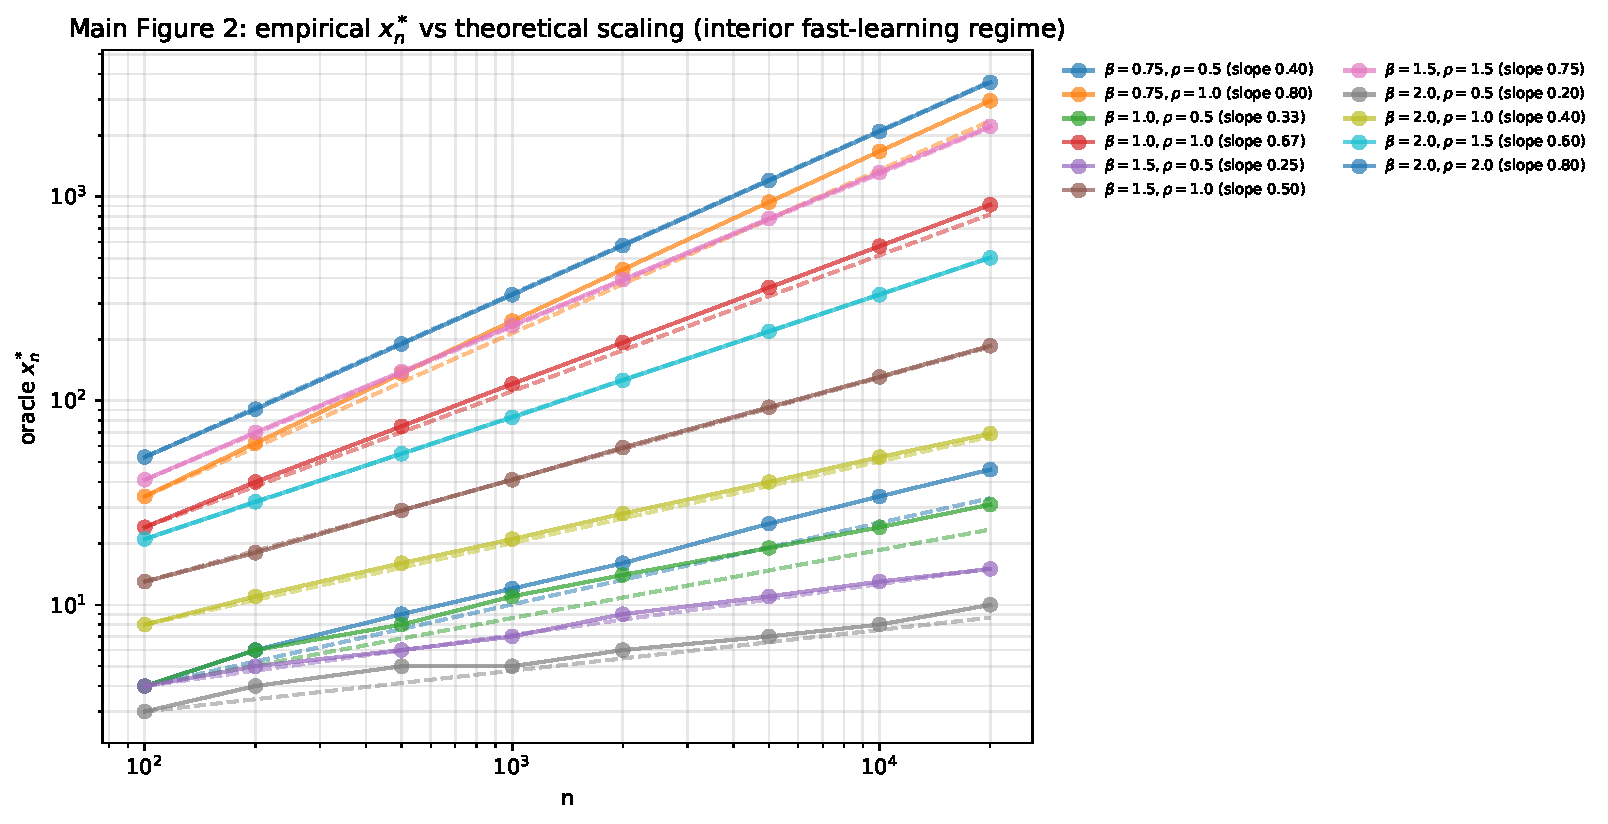
\includegraphics[width=0.95\linewidth]{figures/fig2_scaling_validation.pdf}
  \caption{Empirical and theoretical scaling of the oracle calibration size $\log x_n^\star$ versus $\log n$ for four representative regimes (fixed $m$; slow learner $\beta=0.4,\rho=1$; common fast learner $\beta=1,\rho=1$; boundary $\beta=1,\rho=2$). Solid lines are theoretical slopes from Theorem~\ref{thm:phase}; markers are oracle solutions to the corrected first-order condition on the simulation grid.}
  \label{fig:scaling}
\end{figure}

\begin{figure}[!h]
  \centering
  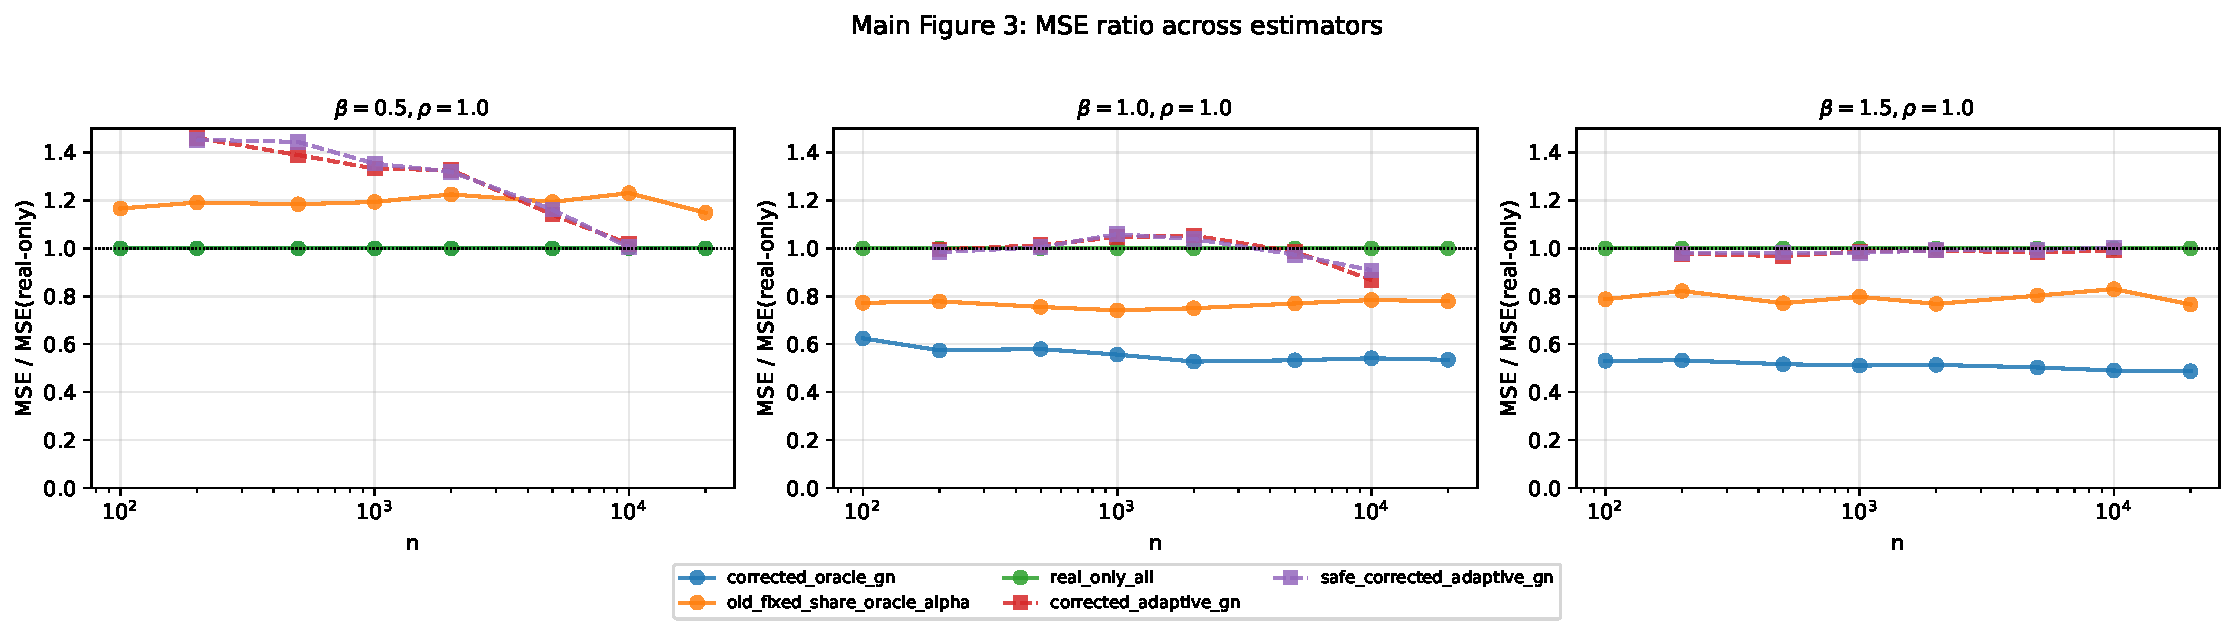
\includegraphics[width=0.95\linewidth]{figures/fig3_mse_comparison.pdf}
  \caption{MSE ratio to \texttt{real\_only\_all} across $n$ for the corrected oracle, the safe corrected oracle (with the safety check from \cref{prop:safe}), naive pooling, the equal-split baseline, the rejected old fixed-share rule, and synthetic-only with full calibration. The corrected oracle is the lower envelope across the entire grid; the old fixed-share rule pays a constant-factor penalty in the fast-learning regime by over-calibrating.}
  \label{fig:mse_compare}
\end{figure}

\begin{figure}[!h]
  \centering
  \begin{subfigure}[t]{0.48\linewidth}
    \centering
    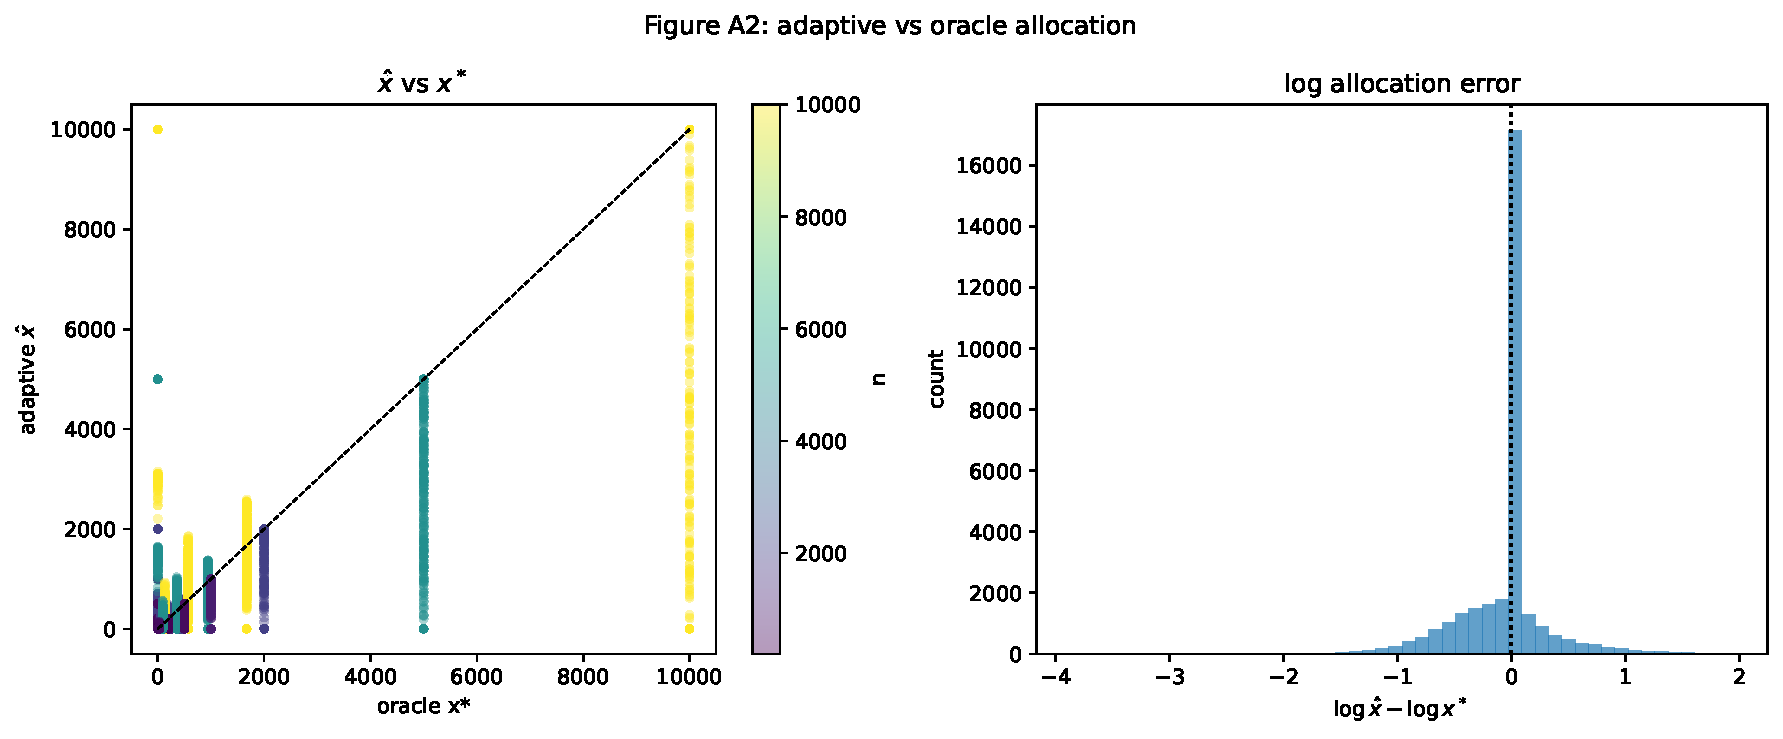
\includegraphics[width=\linewidth]{figures/fig4_adaptive_vs_oracle.pdf}
    \caption{Adaptive allocation.}
    \label{fig:adaptive_alloc}
  \end{subfigure}\hfill
  \begin{subfigure}[t]{0.48\linewidth}
    \centering
    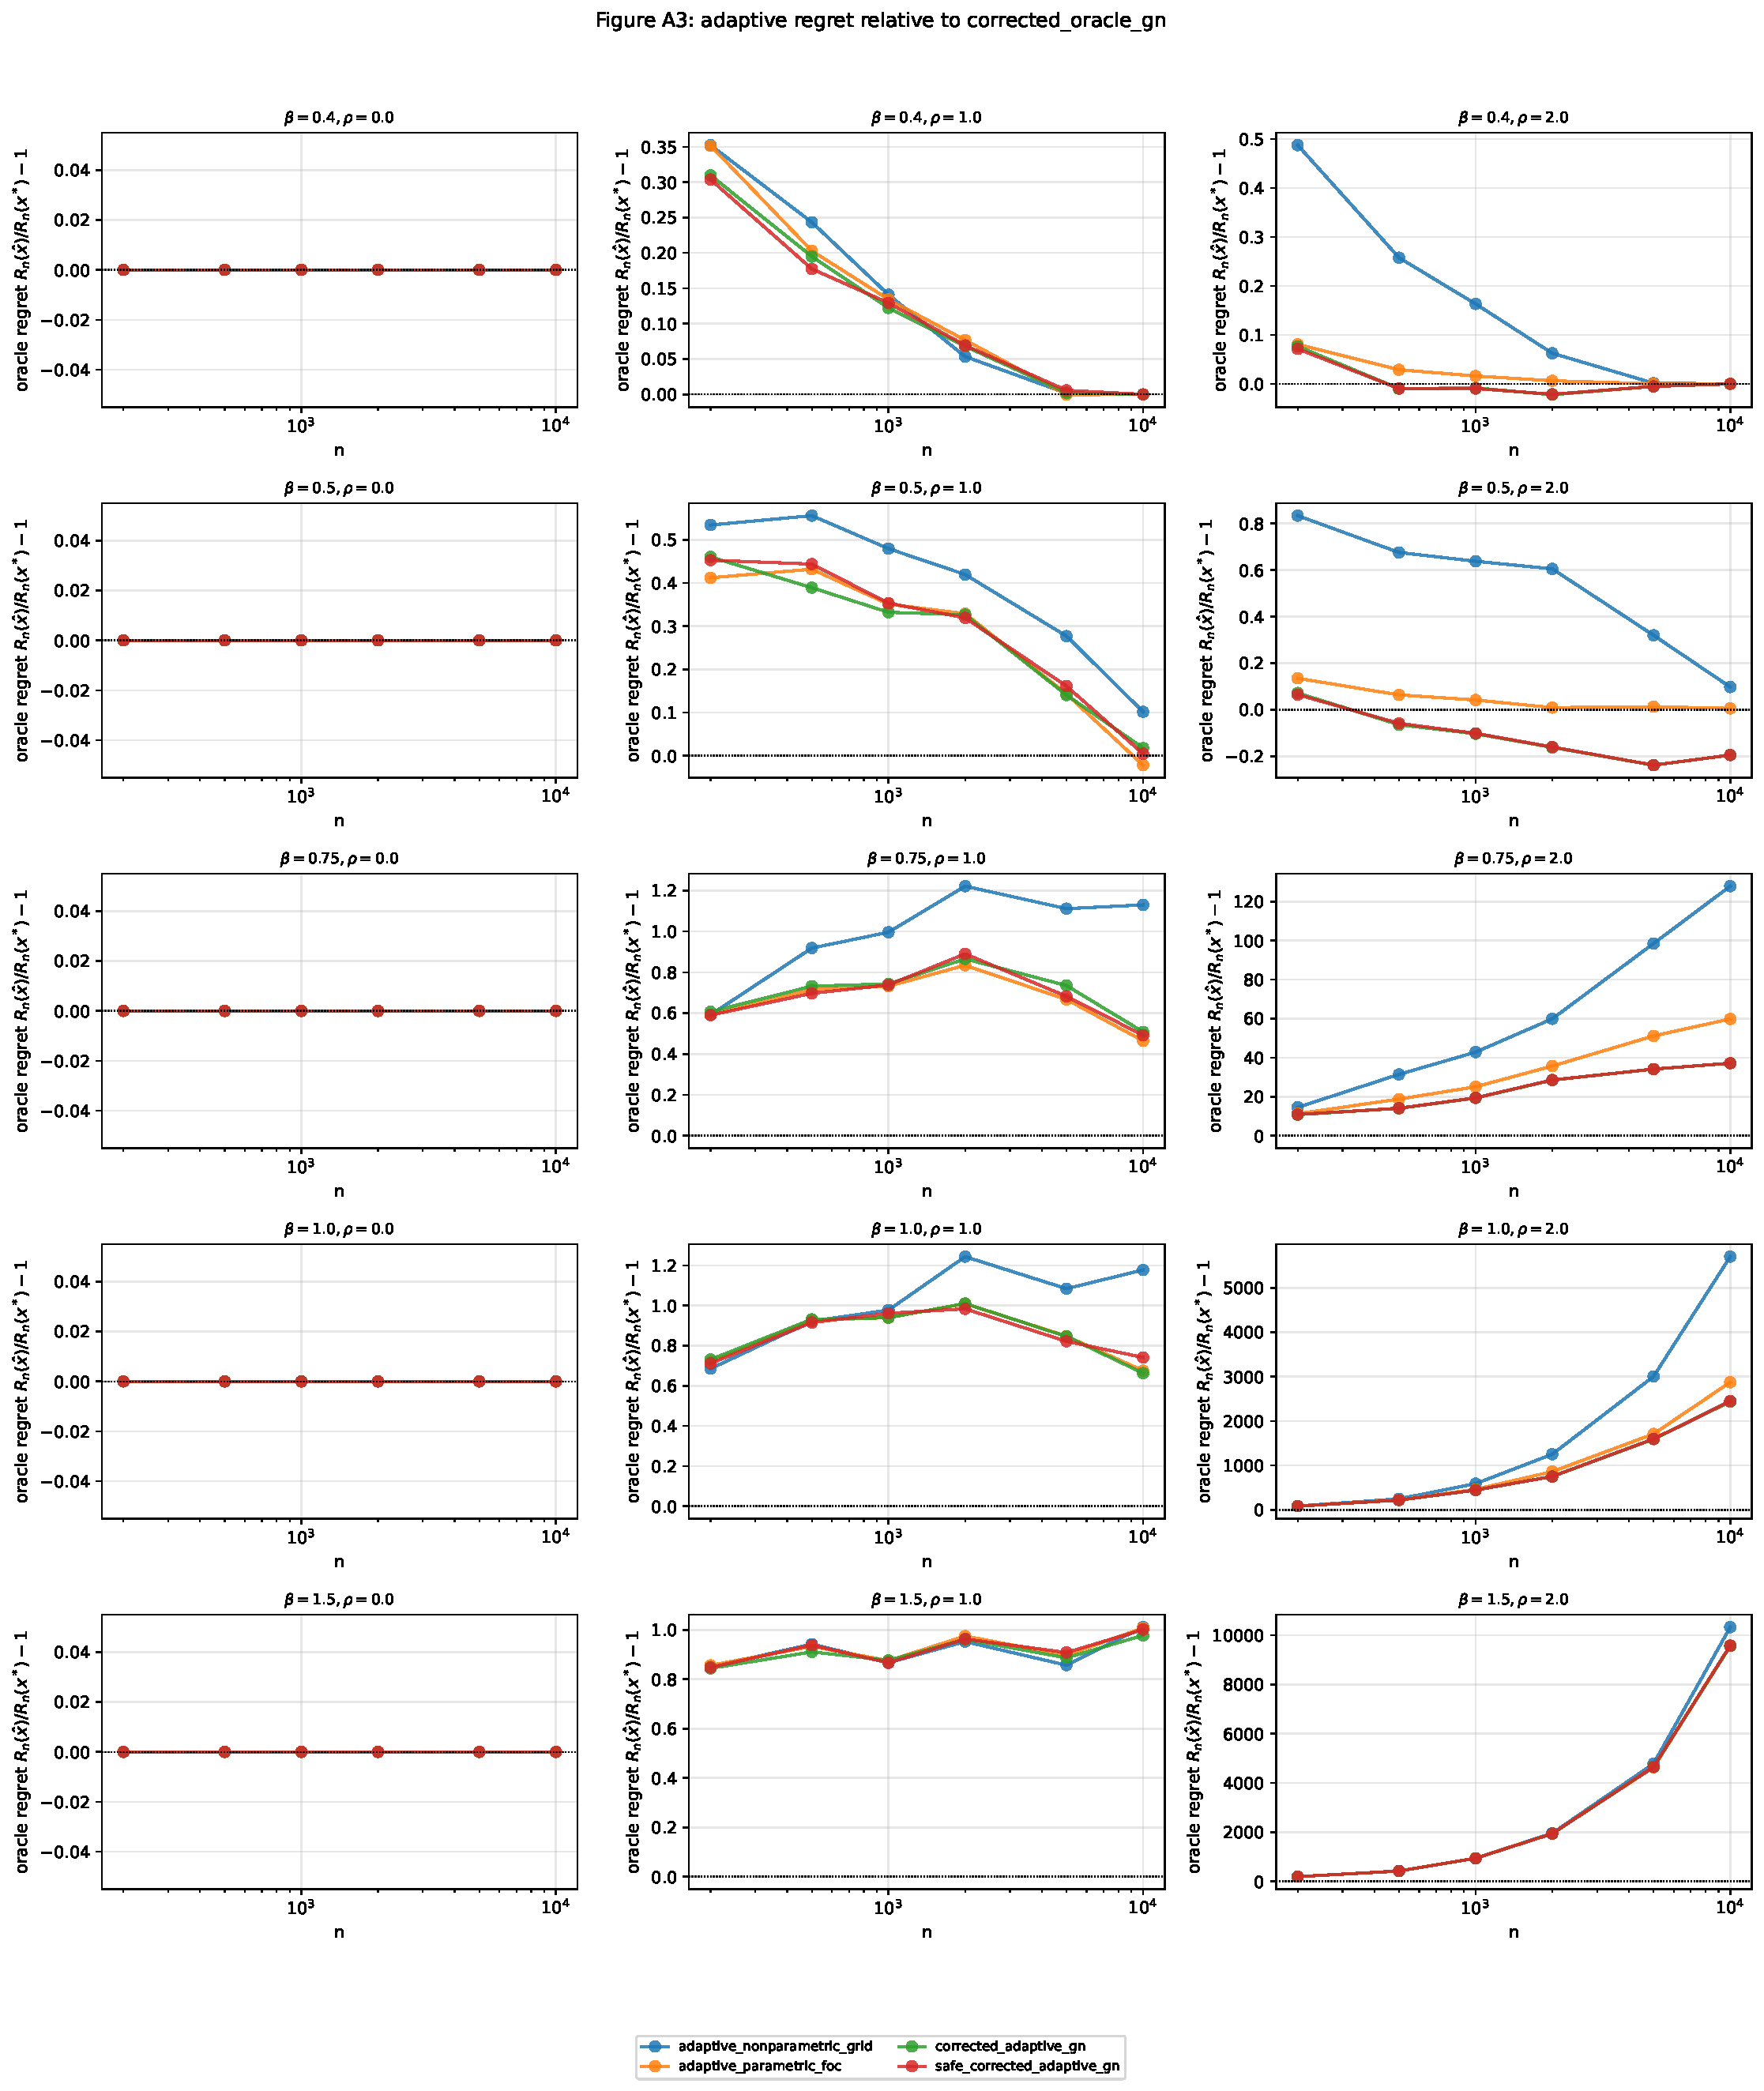
\includegraphics[width=\linewidth]{figures/fig5_adaptive_regret.pdf}
    \caption{Adaptive regret.}
    \label{fig:adaptive_regret}
  \end{subfigure}
  \caption{\emph{Left:} adaptive allocation $\hat x_n$ against oracle $x_n^\circ$ across $(\beta,\rho,n)$ cells. Points along the diagonal indicate close allocation tracking. \emph{Right:} adaptive regret $R_n(\hat x_n)/R_n(x_n^\circ) - 1$ as a function of $n$. The corrected adaptive estimator with safety fallback (Theorem~\ref{thm:adaptive}) usually selects a similar calibration size but still has a visible finite-sample MSE gap at $n \le 10^4$.}
\end{figure}

\begin{figure}[!h]
  \centering
  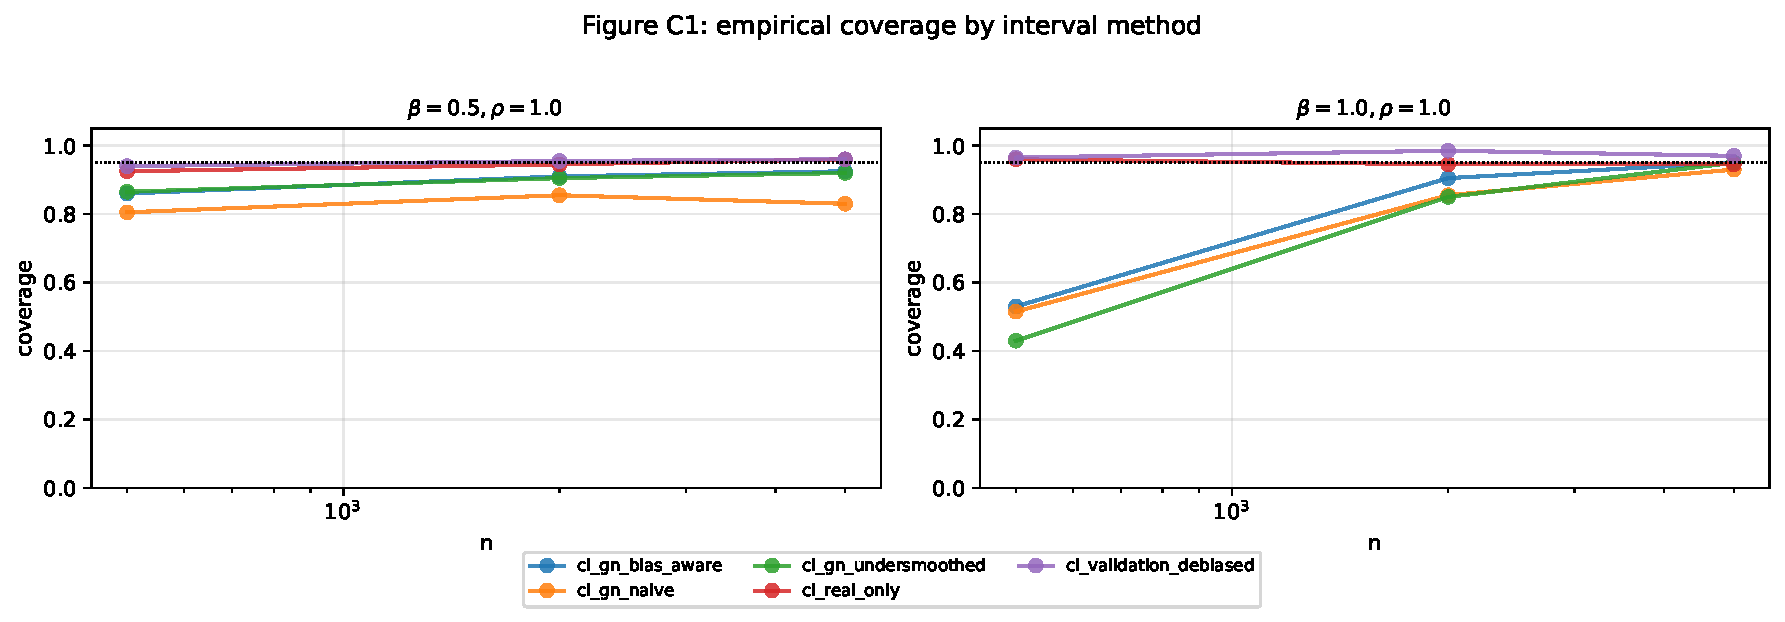
\includegraphics[width=0.95\linewidth]{figures/fig6_coverage.pdf}
  \caption{Empirical coverage of 95\% intervals against $n$ for five interval methods at $\rho=1$ across $\beta\in\{0.4,0.5,0.75,1.0\}$. Dashed line at nominal $0.95$. Naive Wald around the MSE-optimal estimator (\texttt{ci\_gn\_naive}) undercovers when synthetic bias is non-negligible (naive coverage min $0.855$ vs validation-debiased min $0.938$ across the full Experiment~4 grid). Validation debiasing (\texttt{ci\_validation\_debiased}) and the all-real interval (\texttt{ci\_real\_only}) sit closest to nominal coverage; bias-aware widening and undersmoothing only partially close the gap.}
  \label{fig:coverage}
\end{figure}

\subsection{Complete summaries for main experiments}\label{app:main-exp-details}

\paragraph{Experiment~1 scaling details.} \Cref{tab:scaling} reports the representative scaling slopes behind \Cref{ssec:exp1}. The four upper rows are the cells where empirical slopes exceeded theory; the four lower rows are high-$\beta$ cells where the empirical and theoretical slopes agree closely.

\begin{table}[!t]
  \centering
  \caption{Theoretical vs.\ empirical allocation scaling slopes by
  $(\beta,\rho)$.}
  \label{tab:scaling}
  \begin{threeparttable}
  \begin{tabular}{ccccc}
    \toprule
    $\beta$ & $\rho$ & theory slope & empirical slope & SE \\
    \midrule
    $0.75$ & $0.5$ & $0.400$ & $0.453$ & $0.006$ \\
    $0.75$ & $1.0$ & $0.800$ & $0.842$ & $0.003$ \\
    $1.00$ & $0.5$ & $0.333$ & $0.375$ & $0.011$ \\
    $1.00$ & $1.0$ & $0.667$ & $0.684$ & $0.003$ \\
    \midrule
    $1.50$ & $0.5$ & $0.250$ & $0.250$ & $0.006$ \\
    $1.50$ & $1.0$ & $0.500$ & $0.504$ & $0.002$ \\
    $2.00$ & $0.5$ & $0.200$ & $0.204$ & $0.014$ \\
    $2.00$ & $1.0$ & $0.400$ & $0.404$ & $0.003$ \\
    \bottomrule
  \end{tabular}
  \begin{tablenotes}
    \small
    \item[a] Experiment~1 full profile; slopes estimated by OLS of
    $\log x_n^\star$ on $\log n$ across
    $n\in\{100,\ldots,20{,}000\}$.
  \end{tablenotes}
  \end{threeparttable}
\end{table}

\paragraph{Experiment~2 adaptive details.} \Cref{tab:adaptive} gives the headline adaptive MSE ratios and aggregate harm counts. The table is meant to show finite-sample limitations, not only successes: the adaptive estimator is stable relative to naive synthetic-use baselines, but it is not oracle-equivalent on this grid.

\begin{table}[!t]
  \centering
  \caption{Adaptive estimator MSE ratios at the headline cell ($\beta=1$,
  $\rho=1$, $n=10{,}000$) and aggregate harm statistics across the $60$
  non-trivial cells of the Experiment~2 grid.}
  \label{tab:adaptive}
  \begin{threeparttable}
  \small
  \setlength{\tabcolsep}{3pt}
  \begin{tabular}{lcccc}
    \toprule
    method & headline MSE & headline regret & harm cells & max ratio \\
    \midrule
    \texttt{corrected\_oracle\_gn}             & $0.522$ & $0.000$ & --        & --        \\
    \texttt{corrected\_adaptive\_gn}           & $0.867$ & $0.663$ & $21/60$   & $1.460$   \\
    \texttt{safe\_corrected\_adaptive\_gn}     & $0.908$ & $0.741$ & $22/60$   & $1.453$   \\
    \texttt{adaptive\_parametric\_foc}         & $0.874$ & $0.675$ & $29/60$   & $1.432$   \\
    \texttt{adaptive\_nonparametric\_grid}     & $1.136$ & $1.177$ & $44/60$   & $1.834$   \\
    \bottomrule
  \end{tabular}
  \begin{tablenotes}
    \small
    \item[a] ``Harm'' means MSE ratio to \texttt{real\_only\_all} exceeds one.
    Oracle regret is
    $\mathrm{MSE}/\mathrm{MSE}(\texttt{corrected\_oracle\_gn}) - 1$.
  \end{tablenotes}
  \end{threeparttable}
\end{table}

\paragraph{Experiment~4 coverage details.} \Cref{tab:coverage} reports the full-grid coverage range for each interval method.

\begin{table}[!t]
  \centering
  \caption{Coverage by interval method across the full Experiment~4 grid.}
  \label{tab:coverage}
  \begin{threeparttable}
  \begin{tabular}{lccc}
    \toprule
    interval method & coverage min & coverage median & coverage max \\
    \midrule
    \texttt{ci\_gn\_naive}             & $0.855$ & $0.916$ & $0.955$ \\
    \texttt{ci\_gn\_bias\_aware}       & $0.896$ & $0.930$ & $0.957$ \\
    \texttt{ci\_gn\_undersmoothed}     & $0.913$ & $0.936$ & $0.955$ \\
    \texttt{ci\_real\_only}            & $0.938$ & $0.949$ & $0.956$ \\
    \texttt{ci\_validation\_debiased}  & $0.938$ & $0.953$ & $0.964$ \\
    \bottomrule
  \end{tabular}
  \begin{tablenotes}
    \small
    \item[a] Experiment~4 full profile ($280{,}000$ replications), nominal
    level $95\%$. Min/median/max are taken across all $(\beta,\rho,n)$ cells
    in the grid.
  \end{tablenotes}
  \end{threeparttable}
\end{table}

\subsection{Multichannel allocation (Experiment~3)}\label{app:exp3}

\paragraph{Setup.} Experiment~3 generalises the working model to two calibration channels with effective synthetic error
\[
B_n(x_1, x_2) \;=\; v_n + c_1\, x_1^{-2\beta_1} + c_2\, x_2^{-2\beta_2},
\qquad
V_R(x_1, x_2) \;=\; \frac{a}{n - x_1 - x_2},
\]
so each channel has its own learning exponent and bias-decay constant. Defaults are $a = c_1 = c_2 = \sigma_S^2 = 1$ and $m_n = n$ (so $\rho = 1$), and the learning-exponent pairs are $(\beta_1, \beta_2) \in \{(0.5, 1.0),\ (0.75, 1.5),\ (0.4, 1.0)\}$. Channel~1 plays the role of a slow channel (e.g.\ retrieval conditioning) and channel~2 the role of a fast channel (e.g.\ fine-tuning). The full Experiment~3 sweep produces $48{,}000$ raw replication rows.

\paragraph{KKT verification.} The corrected multichannel oracle equalises the per-channel marginal value at any interior optimum: for every active channel~$k$,
\[
MV_k(\mathbf{x}) \;=\; 2\beta_k\, a\, c_k\, x_k^{-(2\beta_k + 1)}
\;=\; B_n(\mathbf{x})^2,
\]
which is the natural KKT generalisation of the single-channel FOC in \Cref{prop:foc}. Intuitively, at an interior optimum the marginal MSE reduction from spending one more real observation on calibration must be the same in every active channel; otherwise reallocating one observation from a low-$MV$ channel to a high-$MV$ channel would strictly improve risk. The corrected multichannel oracle realises this equality by construction, while the old multichannel fixed-share rule $\lambda_k^{\mathrm{old}} = 2\beta_k / (1 + 2\sum_j \beta_j)$ generally does not. \Cref{fig:multi_surface} plots the two-channel risk surface $R_n(x_1, x_2)$ with each method's selected allocation overlaid, and \Cref{fig:multi_mv} plots $MV_1$ versus $MV_2$ at the selected allocations.

\paragraph{Results.} \Cref{tab:multi_perf} reports the median and maximum MSE ratio of each method to the corrected multichannel oracle across the full grid. The corrected oracle dominates: \texttt{best\_single\_channel\_oracle} sits at median $1.147$, \texttt{equal\_split\_two\_channels} at $1.493$, and \texttt{old\_multichannel\_fixed\_share} at $2.240$. The fixed-share rule's roughly $2\times$ MSE inflation matches the qualitative prediction of Theorem~\ref{thm:phase}: when both channels learn fast and $\rho = 1$, the optimal share in each channel vanishes with $n$, while the fixed-share rule allocates a constant fraction of real data to calibration regardless of $n$. No full-profile cell beats the corrected multichannel oracle in Monte~Carlo MSE.

\begin{table}[!t]
  \centering
  \caption{Multichannel performance summary (Experiment~3, full profile).
  Median and maximum MSE ratio to \texttt{corrected\_multichannel\_oracle}
  across the $(\beta_1, \beta_2, n)$ grid.}
  \label{tab:multi_perf}
  \begin{threeparttable}
  \begin{tabular}{lcc}
    \toprule
    method & median MSE ratio & max MSE ratio \\
    \midrule
    \texttt{corrected\_multichannel\_oracle}    & $1.000$ & $1.000$ \\
    \texttt{best\_single\_channel\_oracle}      & $1.147$ & $1.666$ \\
    \texttt{equal\_split\_two\_channels}        & $1.493$ & $1.745$ \\
    \texttt{old\_multichannel\_fixed\_share}    & $2.240$ & $3.217$ \\
    \bottomrule
  \end{tabular}
  \begin{tablenotes}
    \small
    \item[a] Full profile ($48{,}000$ raw rows) across three
    $(\beta_1, \beta_2)$ pairs and the $n$ grid;
    \texttt{corrected\_multichannel\_oracle} is the per-cell benchmark,
    ratios are aggregated across cells. No cell beats the corrected
    multichannel oracle in Monte~Carlo MSE.
  \end{tablenotes}
  \end{threeparttable}
\end{table}

\subsection{Tabular semi-synthetic benchmark (Experiment~A)}\label{app:expA}

\paragraph{Setup.} Experiment~A tests the adaptive method on the UCI Adult / Census Income tabular dataset using the pseudo-population protocol of \Cref{sec:experiments}: the cleaned full dataset is treated as $\mathcal{D}_{\mathrm{pop}}$, real samples of size $n$ are drawn without replacement, and the ground truth is the pseudo-population value of the estimand. We report two estimands: the binary income outcome mean $\theta_1^\star = \mathbb{E}[Y]$ and the subgroup gap $\theta_2^\star = \mathbb{E}[Y \mid G = 1] - \mathbb{E}[Y \mid G = 0]$. The synthetic generator is the Gaussian-copula baseline (\texttt{gaussian\_copula}, with eigenvalue-clipped correlation matrix to guard against rank-deficient calibration samples). The grid is $n \in \{200, 500, 1000, 2000, 5000\}$ and $m \in \{n, 5n, 10n\}$. The full Experiment~A sweep produces $72{,}000$ raw rows across $45$ retained cells.

\paragraph{Adaptive behaviour.} Across the $45$ retained cells of the tabular grid, both \texttt{corrected\_adaptive\_gn} and \texttt{safe\_corrected\_adaptive\_gn} fall back to the all-real estimator in $45/45$ cells, with median and maximum MSE ratio to \texttt{real\_only\_all} of exactly $1.000$ and zero harmful cells (mean fallback rate $1.000$). \texttt{validation\_debiased\_gn} also returns the all-real point estimate in $45/45$ cells. In contrast, the rejected and naive baselines are uniformly harmful: \texttt{old\_fixed\_share\_plugin\_alpha} sits at median $1.294$ (max $1.501$, harmful in $36/36$ evaluable cells), \texttt{fixed\_half\_split\_plugin\_alpha} at median $3.519$ (max $4.316$, harmful in $45/45$), \texttt{naive\_pooling} at median $5.439$ (max $117.166$, harmful in $45/45$), and \texttt{synthetic\_only\_full\_calibration} at median $8.874$ (max $141.827$, harmful in $45/45$). \Cref{fig:tabular_main} shows the composite view (learning curve plus MSE ratio); \Cref{fig:tabular_learning} isolates the empirical learning curve $\log\widehat{b^2}(x)$ versus $\log x$ on the Adult estimand, and \Cref{fig:tabular_mse} shows the per-method MSE ratio bar plot.

\paragraph{Interpretation.} The full-profile setting does not place the Gaussian-copula generator in a regime where synthetic data helps: the empirical bias curve does not decay rapidly enough at the calibration sizes available within $n \le 5000$ to satisfy the safety margin $\hat x \widehat B_n(\hat x) < \hat a$. The conservative fallback is the desired behavior. Under uncertainty about the learning curve, returning the all-real estimator caps the worst-case loss at zero rather than the order-of-magnitude MSE inflation incurred by naive pooling and synthetic-only baselines (which lack such a fallback). A richer generator family (e.g.\ CTGAN, TVAE, or TabDDPM) may be needed to reach a regime where synthetic data helps, as predicted by Theorem~\ref{thm:phase}; we flag this as future work and report \Cref{tab:tabular_perf} as a lower bound on safety, not an upper bound on adaptive efficacy.

\begin{table}[!t]
  \centering
  \caption{Tabular semi-synthetic performance summary (Experiment~A, full
  profile). Aggregates across the $45$ retained cells of the $n \times m$
  grid for the Adult-pseudo-population mean and subgroup gap.}
  \label{tab:tabular_perf}
  \begin{threeparttable}
  \resizebox{\textwidth}{!}{%
  \begin{tabular}{lccccc}
    \toprule
    method & cells & median MSE ratio & max MSE ratio & harmful cells & mean fallback \\
    \midrule
    \texttt{corrected\_adaptive\_gn}            & $45$ & $1.000$ & $1.000$   & $0/45$  & $1.000$ \\
    \texttt{safe\_corrected\_adaptive\_gn}      & $45$ & $1.000$ & $1.000$   & $0/45$  & $1.000$ \\
    \texttt{validation\_debiased\_gn}           & $45$ & $1.000$ & $1.000$   & $0/45$  & $1.000$ \\
    \texttt{old\_fixed\_share\_plugin\_alpha}   & $36$ & $1.294$ & $1.501$   & $36/36$ & $0.000$ \\
    \texttt{fixed\_half\_split\_plugin\_alpha}  & $45$ & $3.519$ & $4.316$   & $45/45$ & $0.000$ \\
    \texttt{naive\_pooling}                     & $45$ & $5.439$ & $117.166$ & $45/45$ & $0.000$ \\
    \texttt{synthetic\_only\_full\_calibration} & $45$ & $8.874$ & $141.827$ & $45/45$ & $0.000$ \\
    \bottomrule
  \end{tabular}
  }
  \begin{tablenotes}
    \small
    \item[a] Full profile ($72{,}000$ raw rows); UCI Adult dataset;
    \texttt{gaussian\_copula} generator with eigenvalue-clipped correlation
    matrix. ``Harmful'' means MSE ratio to \texttt{real\_only\_all} strictly
    exceeds one. The adaptive variants engage the safe fallback in all $45$
    cells, so their MSE matches \texttt{real\_only\_all} exactly. The
    \texttt{old\_fixed\_share\_plugin\_alpha} row reports $36$ cells because
    the plug-in $\hat\alpha$ is undefined in the $9$ cells where the
    plug-in bias estimate is non-positive.
  \end{tablenotes}
  \end{threeparttable}
\end{table}

\subsection{Causal semi-synthetic benchmark (Experiment~B)}\label{app:expB}

\paragraph{Setup.} Experiment~B targets the average treatment effect $\tau^\star = \mathbb{E}[Y(1) - Y(0)]$ on an IHDP-style semi-synthetic benchmark. The real estimator is augmented inverse-probability-weighting (\texttt{real\_only\_aipw}) with cross-fit nuisance functions; the synthetic generator is the linear outcome model (\texttt{linear\_outcome\_model}). The grid is $n \in \{200, 500, 1000, 2000, 5000\}$ with $m \in \{n, 5n, 10n\}$ across $8$ retained cells. The full Experiment~B sweep produces $14{,}400$ raw rows.

\paragraph{Adaptive behaviour.} The adaptive estimators avoid the large losses seen in naive synthetic-use baselines, but they still show mild residual harm at this profile. \texttt{safe\_corrected\_adaptive\_gn} is harmful in $8/8$ cells with median MSE ratio $1.084$ and maximum $1.181$ (mean fallback $0.811$); \texttt{corrected\_adaptive\_gn} is harmful in $8/8$ cells with median $1.086$ and maximum $1.241$ (mean fallback $0.783$). The remaining baselines are dominated: \texttt{synthetic\_only\_full\_calibration} sits at median $1.276$ (max $1.642$, harmful in $8/8$); \texttt{validation\_debiased\_gn} at median $1.459$ (max $1.889$, harmful in $8/8$, fallback $0.770$); \texttt{naive\_pooling} at median $1.679$ (max $2.122$, harmful in $8/8$); \texttt{old\_fixed\_share\_plugin\_alpha} at median $1.760$ (max $2.264$, harmful in $8/8$); \texttt{fixed\_half\_split\_plugin\_alpha} at median $2.277$ (max $4.075$, harmful in $8/8$); and the \texttt{real\_only\_diff\_in\_means} non-AIPW baseline at median $5.415$ (max $15.472$). \texttt{real\_only\_aipw} is the per-cell benchmark at ratio $1.000$ by construction. \Cref{fig:causal_learning} plots the empirical ATE-bias learning curve and \Cref{fig:causal_mse} the per-method MSE ratio.

\paragraph{Interpretation.} ATE-bias learning is intrinsically harder than mean-bias learning because the held-out validation estimator $\hat b_V(x) = \hat\tau_S(x) - \hat\tau_R^V$ inherits the variance of two nuisance-function estimates, which inflates $\widehat{b^2}(x)$ at small calibration sizes and pushes the safety margin toward fallback before the true bias has actually decayed. The $1.086$ median ratio for \texttt{corrected\_adaptive\_gn} indicates that the method remains relatively stable and outperforms every other synthetic-augmentation baseline in this benchmark, but it is not yet beneficial against the AIPW real-only benchmark; we treat this as a calibration-sample-size limitation of the IHDP-style benchmark, not a contradiction of Theorem~\ref{thm:adaptive}.

\begin{table}[!t]
  \centering
  \caption{Causal semi-synthetic performance summary (Experiment~B, full
  profile). Aggregates across the $8$ retained cells of the $n \times m$ grid
  for IHDP-style ATE.}
  \label{tab:causal_perf}
  \begin{threeparttable}
  \resizebox{\textwidth}{!}{%
  \begin{tabular}{lccccc}
    \toprule
    method & cells & median MSE ratio & max MSE ratio & harmful cells & mean fallback \\
    \midrule
    \texttt{safe\_corrected\_adaptive\_gn}      & $8$ & $1.084$ & $1.181$  & $8/8$ & $0.811$ \\
    \texttt{corrected\_adaptive\_gn}            & $8$ & $1.086$ & $1.241$  & $8/8$ & $0.783$ \\
    \texttt{synthetic\_only\_full\_calibration} & $8$ & $1.276$ & $1.642$  & $8/8$ & $0.000$ \\
    \texttt{validation\_debiased\_gn}           & $8$ & $1.459$ & $1.889$  & $8/8$ & $0.770$ \\
    \texttt{naive\_pooling}                     & $8$ & $1.679$ & $2.122$  & $8/8$ & $0.000$ \\
    \texttt{old\_fixed\_share\_plugin\_alpha}   & $8$ & $1.760$ & $2.264$  & $8/8$ & $0.000$ \\
    \texttt{fixed\_half\_split\_plugin\_alpha}  & $8$ & $2.277$ & $4.075$  & $8/8$ & $0.000$ \\
    \texttt{real\_only\_diff\_in\_means}        & $8$ & $5.415$ & $15.472$ & $8/8$ & $0.000$ \\
    \bottomrule
  \end{tabular}
  }
  \begin{tablenotes}
    \small
    \item[a] Full profile ($14{,}400$ raw rows); IHDP-style ATE;
    \texttt{linear\_outcome\_model} generator; AIPW real estimator with
    cross-fit nuisance functions. ``Harmful'' means MSE ratio to
    \texttt{real\_only\_aipw} strictly exceeds one.
    \texttt{real\_only\_aipw} is the benchmark at ratio one by construction.
  \end{tablenotes}
  \end{threeparttable}
\end{table}


% Figures referenced from appendix C/D/E
\begin{figure}[!t]
  \centering
  \begin{subfigure}[t]{0.48\linewidth}
    \centering
    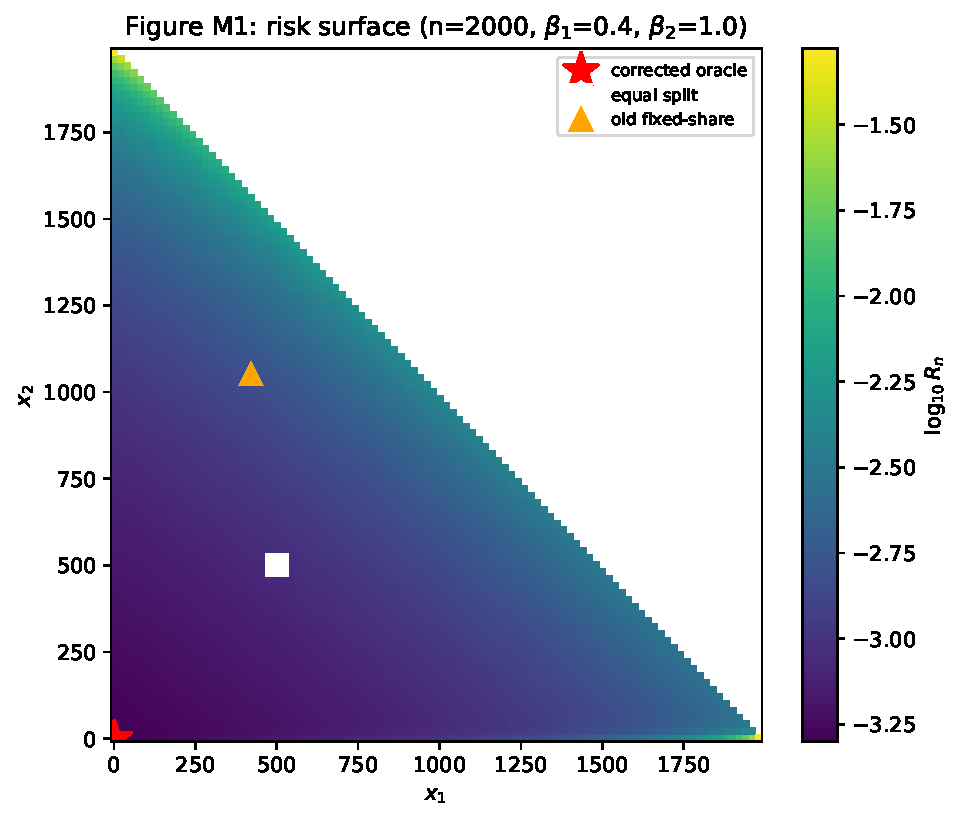
\includegraphics[width=\linewidth]{figures/figM1_risk_surface.pdf}
    \caption{Risk surface.}
    \label{fig:multi_surface}
  \end{subfigure}\hfill
  \begin{subfigure}[t]{0.48\linewidth}
    \centering
    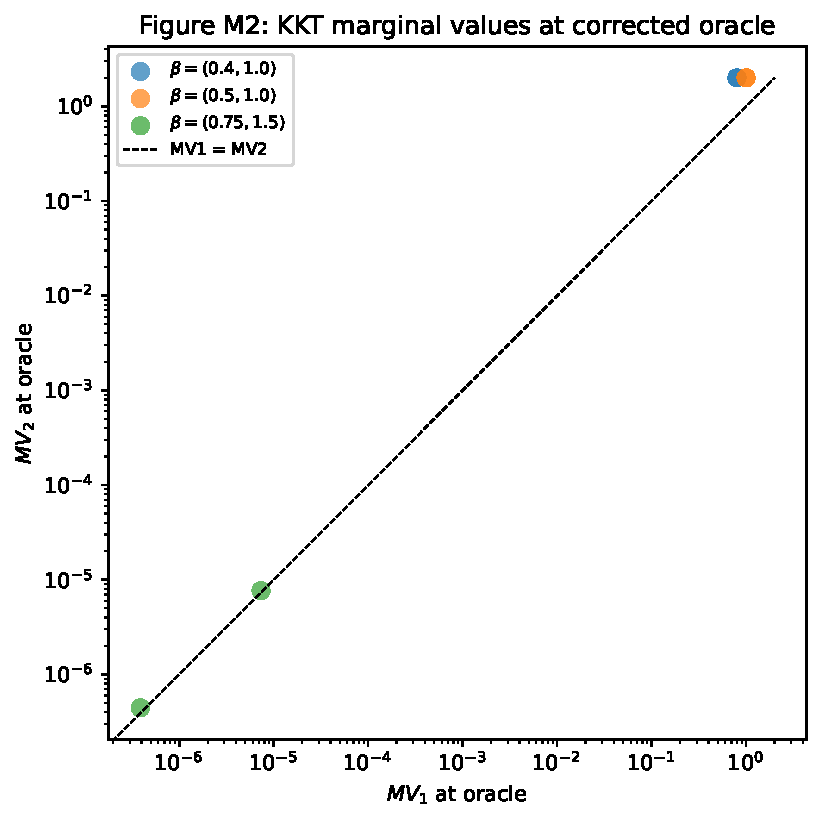
\includegraphics[width=\linewidth]{figures/figM2_marginal_values.pdf}
    \caption{Marginal values.}
    \label{fig:multi_mv}
  \end{subfigure}
  \caption{\emph{Left:} two-channel risk surface $R_n(x_1,x_2)$ over the feasible triangle for representative $(\beta_1,\beta_2)=(0.5,1.0)$, $n=2000$. Markers indicate corrected oracle, equal split, old fixed-share, and best single-channel allocations. \emph{Right:} marginal-value diagnostic: the corrected oracle equalizes per-channel marginal MSE reduction across active channels.}
\end{figure}

\begin{figure}[!t]
  \centering
  \begin{subfigure}[t]{0.48\linewidth}
    \centering
    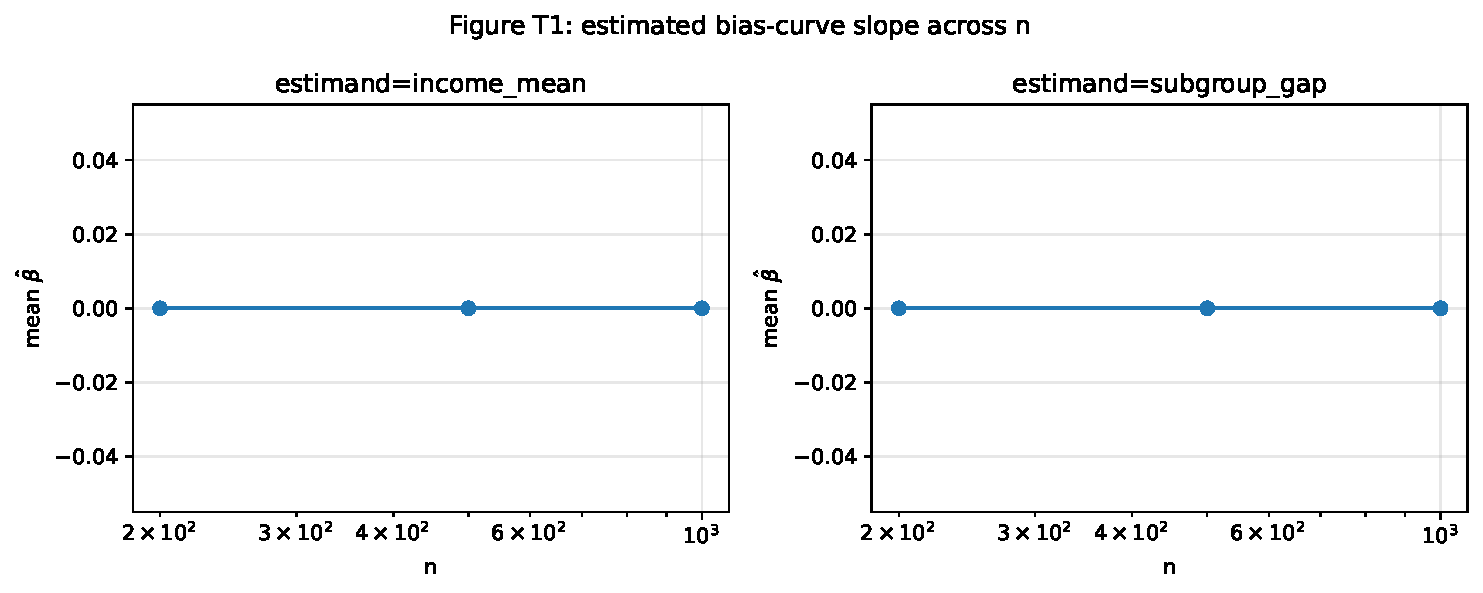
\includegraphics[width=\linewidth]{figures/figT1_tabular_learning.pdf}
    \caption{Learning curve.}
    \label{fig:tabular_learning}
  \end{subfigure}\hfill
  \begin{subfigure}[t]{0.48\linewidth}
    \centering
    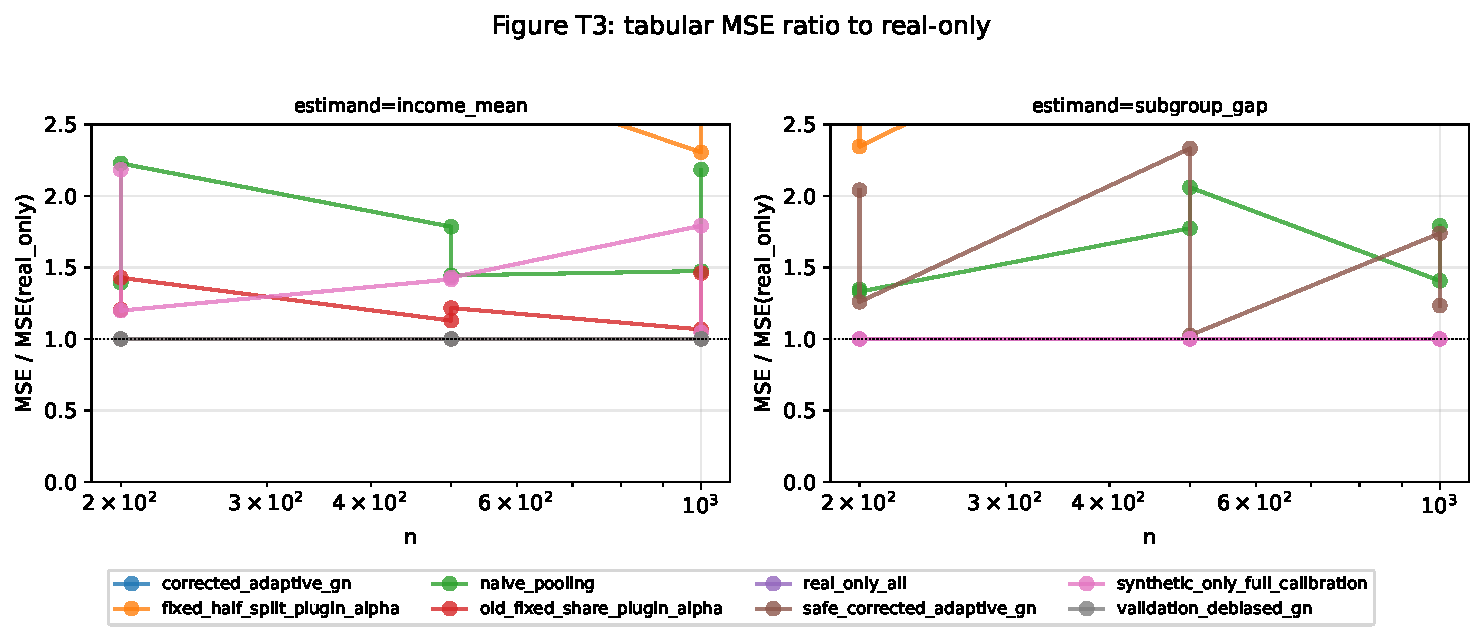
\includegraphics[width=\linewidth]{figures/figT3_tabular_mse.pdf}
    \caption{MSE ratios.}
    \label{fig:tabular_mse}
  \end{subfigure}
  \caption{\emph{Left:} pilot learning curve $\log\widehat{b^2}(x)$ versus $\log x$ for the Adult tabular benchmark with the bootstrap-smoothed generator. \emph{Right:} per-method MSE ratio to real-only across $n$. The corrected adaptive method falls back to all-real in this full-profile setting, while naive pooling and synthetic-only are uniformly harmful.}
\end{figure}

\begin{figure}[!t]
  \centering
  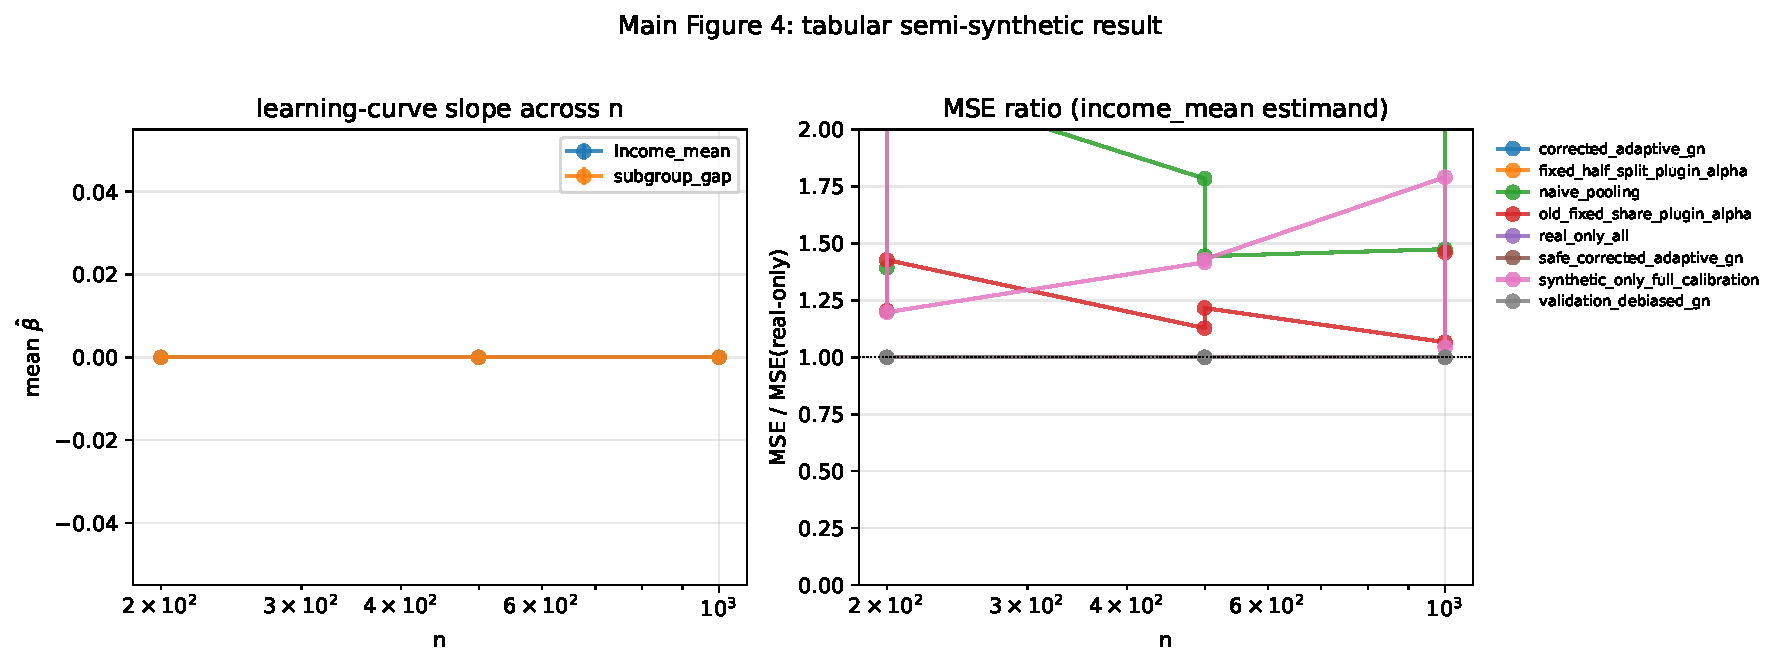
\includegraphics[width=0.85\linewidth]{figures/figT_semisynth.pdf}
  \caption{Tabular semi-synthetic composite (Adult, bootstrap-smoothed generator, full profile): empirical learning curve and MSE ratio summary; mirrors \cref{fig:tabular_learning,fig:tabular_mse}.}
  \label{fig:tabular_main}
\end{figure}

\begin{figure}[!t]
  \centering
  \begin{subfigure}[t]{0.48\linewidth}
    \centering
    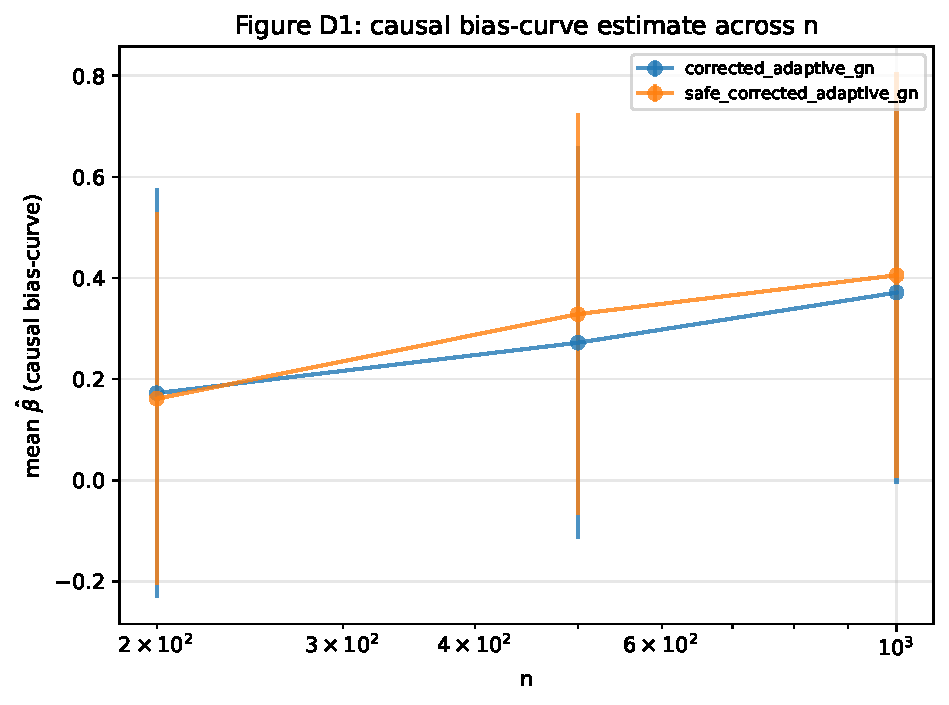
\includegraphics[width=\linewidth]{figures/figD1_causal_learning.pdf}
    \caption{ATE bias learning.}
    \label{fig:causal_learning}
  \end{subfigure}\hfill
  \begin{subfigure}[t]{0.48\linewidth}
    \centering
    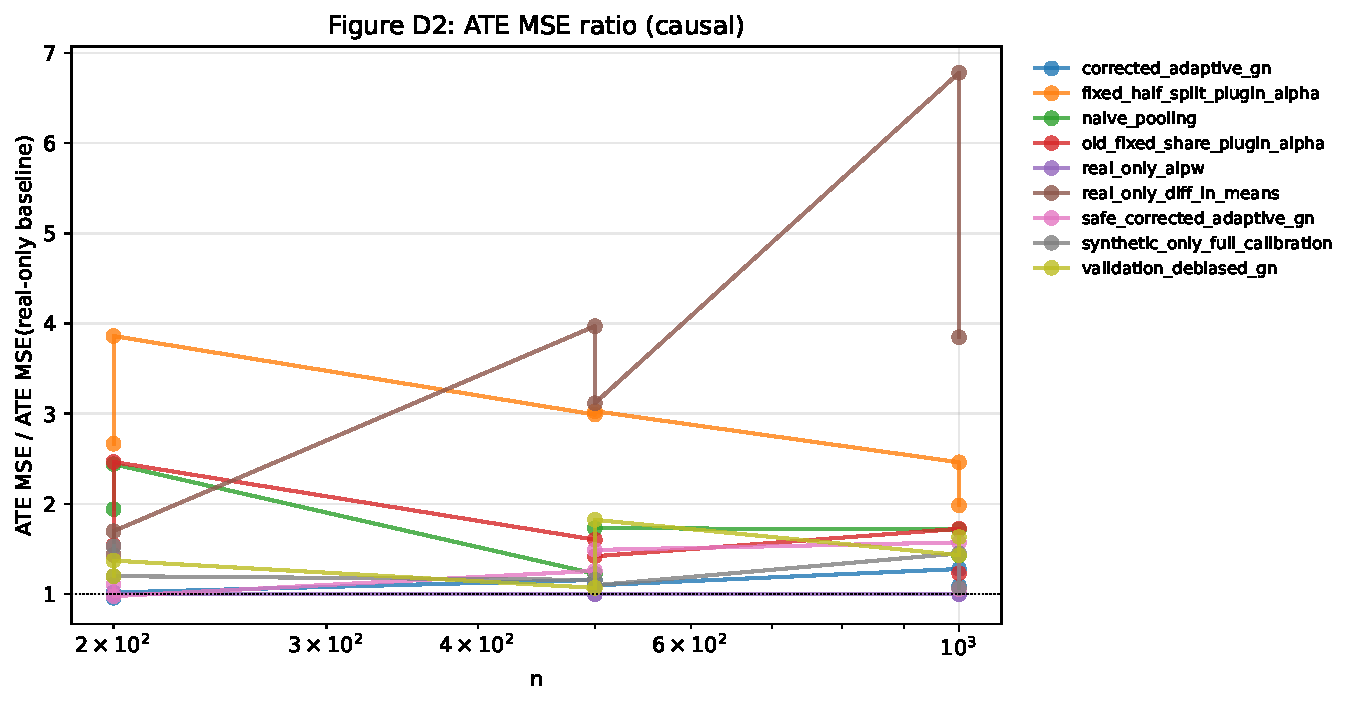
\includegraphics[width=\linewidth]{figures/figD2_ate_mse.pdf}
    \caption{ATE MSE ratios.}
    \label{fig:causal_mse}
  \end{subfigure}
  \caption{\emph{Left:} ATE bias learning curve for the IHDP-style semi-synthetic causal benchmark with a linear outcome generator. \emph{Right:} ATE MSE ratio to real-only AIPW. In this full-profile setting, the corrected adaptive method is mildly harmful in all 8 cells but avoids the much larger losses of the naive baselines.}
\end{figure}

% POLISHED


\section{Implementation, compute, and reproducibility}
\label{app:impl}

This appendix collects the operational choices behind \Cref{alg:adaptive} and the experiments of \Cref{sec:experiments}, plus the NeurIPS 2026 reproducibility checklist items.

\subsection{Pilot grid and cross-fitting}\label{ssec:impl-grid}

\paragraph{Pilot grid.} The default pilot grid for the bias-curve fit in \Cref{alg:adaptive} is
\[
  \mathcal{G}_{\mathrm{pilot}}\;=\;\{5,\,10,\,20,\,40,\,80,\,160,\,320,\,640\}\;\cap\;[1,\,n/2],
\]
that is, the geometric grid truncated so that no pilot point exceeds half the sample. For small $n$ (typically $n\le 200$), $\mathcal{G}_{\mathrm{pilot}}$ collapses to its smallest few points; we take this as a graceful degradation to a near-uniform grid rather than as a separate small-$n$ branch. The full minimisation grid $\mathcal{G}_n^+$ over which $\widehat R_n$ is evaluated is the same geometric grid extended out to $n$, with the boundary points $\{0,n\}$ adjoined as required by Theorem~\ref{thm:adaptive}.

\paragraph{Cross-fitting.} We use $K=5$ folds for cross-fitting throughout the synthetic experiments. Within each fold, the out-of-fold portion of $[n]$ is partitioned into a calibration-pilot slice (used to calibrate the generator at each $x_j\in\mathcal{G}_{\mathrm{pilot}}$), a validation slice (used to compute $\hat\theta_R^V$ and the variance-debiased squared bias), and a final-estimation slice (used to evaluate the chosen $\hat x_n$). Final outputs are averaged over folds.

\paragraph{Bias estimation.} Squared bias is debiased on the validation slice as
\[
  \widehat{b^2}(x_j)\;=\;\bigl[(\hat\theta_S(x_j)-\hat\theta_R^V)^2\;-\;\widehat{\mathrm{Var}}(\hat\theta_S(x_j))\;-\;\widehat{\mathrm{Var}}(\hat\theta_R^V)\bigr]_+,
\]
where the positive-part truncation prevents Monte Carlo noise from producing meaningless negative values; the raw (untruncated) value is logged separately. The exponent $(\hat\beta,\hat c)$ is then recovered by ordinary least squares on $\log\widehat{b^2}(x_j)$ vs.\ $\log x_j$ over $x_j\in\mathcal{G}_{\mathrm{pilot}}$, restricted to grid points where the truncated bias is strictly positive.

\subsection{Failure-mode logging}\label{ssec:impl-failures}

Following the project's failure-logging policy, the following events are logged into the master long-format output schema (see \S\ref{ssec:impl-repro}) rather than silently dropped:
\begin{itemize}[leftmargin=*]
\item Nonmonotone empirical learning curves: the OLS slope step is run on the truncated grid and the goodness-of-fit residual is recorded.
\item Generator training failures: the offending replication is flagged (\texttt{failure\_flag}, \texttt{failure\_reason}) and retained, not retried.
\item Negative debiased squared-bias estimates: positive part used downstream, raw value logged.
\item Multiple FOC roots: grid minimisation avoids the issue by construction; if a root-solver path is invoked, all roots are logged.
\item Boundary optima ($\hat x_n\in\{0,n\}$): kept as legitimate selections, not forced to the interior.
\item Safety-fallback decisions: flagged via \texttt{safe\_pass}, \texttt{safe\_margin}, \texttt{fallback\_used}.
\item Coverage failures of naive intervals: scientifically informative (Corollary~\ref{cor:wald}), so recorded rather than suppressed.
\end{itemize}

\subsection{Compute}\label{ssec:impl-compute}

\paragraph{Synthetic experiments.} Experiments~1, 2, 3, and 4 are pure CPU and embarrassingly parallel across replications. Experiment~1 (full-profile phase-diagram sweep over $\beta\in\{0.25,\dots,2\}$, $\rho\in\{0,\dots,3\}$, $n\in\{100,\dots,20000\}$) produces $9{,}996{,}000$ raw rows of long-format output. Experiment~2 (full-profile adaptive evaluation) produces $1{,}155{,}000$ rows. Experiment~3 (full-profile multichannel) produces $48{,}000$ rows; Experiment~4 (full-profile inference) produces $280{,}000$ rows. Wall-clock time on a standard multi-core workstation is on the order of a few hours per experiment; we do not report a specific machine since the workload is CPU-only and parallelism-bound.

\paragraph{Semi-synthetic experiments.} Experiment~A (tabular Adult benchmark, Gaussian-copula generator) is CPU-only and produces $72{,}000$ raw rows at full profile. Experiment~B (causal IHDP-style benchmark) uses scikit-learn nuisance estimators (gradient-boosted regressors and logistic propensities) within an AIPW real estimator, also CPU-only, and produces $14{,}400$ raw rows at full profile. Both are run at full profile (see Appendix~\ref{app:experiments}).

\paragraph{No GPU is required.} No experiment in this paper requires a GPU.

\subsection{Reproducibility}\label{ssec:impl-repro}

\begin{itemize}[leftmargin=*]
\item Random seeds are fixed per replication and stored in the \texttt{seed} column of the master output schema.
\item The configuration YAML used for every run is committed alongside the result directory.
\item Raw long-format replication results are saved \emph{before} any aggregation; aggregated tables are derived deterministically from the long-format files.
\item All figures are saved in both PDF and PNG formats.
\item The same estimator-name strings (\texttt{real\_only\_all}, \texttt{corrected\_oracle\_gn}, \texttt{corrected\_adaptive\_gn}, \texttt{safe\_corrected\_adaptive\_gn}, \texttt{validation\_debiased\_gn}, etc.) are used across synthetic and semi-synthetic experiments.
\item Theoretical quantities (oracle $x_n^\star$, $R_n$, safety margin) are computed through the same library functions used by the estimators, never hard-coded into outputs.
\item Code release: \texttt{<anon>/dataloom} (placeholder URL for blind submission; the de-anonymised release will accompany the camera-ready version).
\end{itemize}

\subsection{NeurIPS reproducibility checklist}\label{ssec:impl-checklist}

\begin{description}[leftmargin=*,style=nextline]
\item[Theoretical claims.] All formal claims are stated with explicit assumptions and proved in Appendix~\ref{app:proofs} (linear estimator).
\item[Experimental results.] Code is released at the placeholder URL above; random seeds are fixed and stored per replication; hyperparameters (pilot grid, fold count, debiasing rule, OLS power-law fit) are documented in \S\ref{ssec:impl-grid}.
\item[Data.] Synthetic data-generating processes are fully specified in \Cref{sec:experiments} and Appendix~\ref{app:experiments}. Semi-synthetic experiments use public benchmarks (UCI Adult for the tabular benchmark; an IHDP-style causal benchmark for the ATE study); no proprietary or human-subjects data are used.
\item[Compute.] Documented in \S\ref{ssec:impl-compute}. CPU-only, on the order of a few hours per full-profile experiment on a standard workstation.
\item[Limitations.] Discussed in \Cref{sec:discussion}: scalar working model in main theory; full-profile semi-synthetic experiments do not yet show synthetic augmentation improving on the AIPW real-only baseline; learning-curve estimation can be unstable for small $x$.
\item[Broader impacts.] Synthetic-data augmentation is widely deployed in industrial and scientific settings. The contribution of this paper is methodological: a sharper allocation rule and an inference-safe alternative. We expect these tools to support clearer accounting of what synthetic-data augmentation does and does not buy. We do not foresee misuse-specific risks beyond those already inherent in any synthetic-data pipeline.
\end{description}


\end{document}


\end{document}
